\chapter{Reduction of the Kirchhoff Rod} \label{chap:reduction}
%
In this chapter the Casimirs of the Kirchhoff equations are used to reduce the noncanonical Hamiltonian system to a lower dimensional canonical system, allowing for a range of analytic tools to be applied. In the integrable Lagrange case planar phase diagrams are computed and fixed point and homoclinic solutions found. The reduction allows some nonintegrable perturbations to be expressed in a way that allows Poincar\'e sections to be computed. Mel'nikov's method is then appplied to show that anisotropic and initially curved rods are not completely integrable and the loss of integrability is accompanied by Smale horseshoes on the Poincar\'e sections of the homoclinic energy level. The consequences of nonintegrability in these two cases are then outlined.
%
\section{Reduction to a Canonical System}
%
In this section the two Casimirs of the Kirchhoff equation~\eqref{eq:kirchoff_casimirs} are used to reduce the six-dimensional non-canonical Hamiltonian system~\eqref{eq:kirchhoff_bracket} to a four-dimensional canonical Hamiltonian system using Euler angles~\eqref{eq:euler_angles}, where the canonical coordinates are $q=\left(\theta,\phi,\psi\right)$ and their conjugate momenta $p=\left(p_{\theta},p_{\phi},p_{\psi}\right)$. This is possible (at least locally) provided the structure matrix~\eqref{eq:kirchhoff_structure} is of constant rank everywhere~\cite[\S{6.2}]{Olver93}. The key to the analysis is that the angles~$\left(\phi,\psi\right)$ and their conjugate momenta~$\left(p_{\phi},p_{\psi}\right)$ are action-angle variables as the integrals represented are both associated with rotational symmetry. 
% Thus in the isotropic case the system can be reduced to an equivalent oscillator on the phase space $T^{*}S^{1}$.
% 
\par
However, before the reduction can be performed, the system is nondimensionalised. Let a torque, $M$, and tension, $T$, be applied in the direction of $\boldsymbol{d}_{3}$ at $s=\pm\infty$. By scaling the arclength by $t=\left(M/B_{1}\right)$, where $B_{1}$ is one of the principal bending stiffnesses and scaling the force and moments by 
% 
\begin{align}
\bar{m}_{1} & = m_{1} \slash M, \quad \bar{m}_{2} = m_{2} \slash M, \quad \bar{m}_{3} = \left( m_{3}-1 \right) \slash M, \nonumber \\
\bar{n}_{1} & = n_{1}\slash T, \quad \bar{n}_{2} = n_{2}\slash T \quad \mbox{and} \quad \bar{n}_{3} = \left(n_{3}-1\right)\slash T \nonumber
\end{align}
% 
the system is nondimensional. Then from the general constitutive relations~\eqref{eq:hyperelastic}, the following nondimensional parameters emerge
%
\begin{equation}
\begin{array}{c}
m = \dfrac{M}{\sqrt{B_{2}T}}, \quad \rho = \dfrac{B_{2}}{B_{1}}-1, \quad \nu = \dfrac{B_{2}}{C}-1,  \\
\quad \epsilon = \dfrac{T}{J}, \quad \sigma = \dfrac{J}{H}-1, \quad \gamma = \dfrac{K}{J}-1 \quad \mbox{and} \quad \kappa_{0} = \dfrac{B_{1}u_{0}}{M}. 
\end{array} \label{eq:nondim}
\end{equation}
%
Where $m$ is the unified end loding parameter, $\rho$ the degree of isotropy, $\nu$ the rate of torsional stiffness to bending stiffness, $\epsilon$ measures the importance of shear with respect to bending, $\gamma$ and $\sigma$ are the analogues of $\rho$ and $\nu$ for extensibility and shear and $\kappa_{0}$ the degree of initial curvature. Without loss of generality dropping the overbar for the nondimensional force and moments, then the nondimensional inextensible and unshearable Hamiltonian is given by
% 
\begin{align}
\mathcal{H} & = \frac{1}{2}\left(1+\rho\right)m_{1}^{2} + \frac{1}{2}m_{2}^{2} + \frac{1}{2}\left(1+\nu\right)m_{3}^{2} + \frac{n_{3}}{m^{2}}. \nonumber
\end{align}
% 
\par
Let
%
\begin{align}
R & = 
\left(
\begin{array}{ccc}
\cos\theta\cos\phi\cos\psi-\sin\phi\sin\psi & \cos\theta\cos\phi\sin\psi+\cos\psi\sin\phi & -\sin\theta\cos\phi \\
-\cos\theta\sin\phi\cos\psi-\cos\phi\sin\psi & -\cos\theta\sin\phi\sin\psi+\cos\phi\cos\psi & \sin\theta\sin\phi \\
\sin\theta\cos\psi & \sin\theta\sin\psi & \cos\theta
\end{array}
\right)
\nonumber
\end{align}
%
be a parametrisation of the rotation matrix~\eqref{eq:frame} in terms of Euler angles. Following the convention used by Love~\cite{Love44}, here $\theta$ is the angle the tangent to the rod makes with the initially straight rod, $\psi$ is the azimuthal angle about a fixed axis and $\phi$ is the twist angle about the centreline of the rod.  Using the Euler angles and expression of the strains~\eqref{eq:curvatures}, the strains ${u}_{i}\left(q,q^{\prime}\right)$ are given by
%
\begin{subequations}
\label{eq:strains}
\begin{align}
u_{1} & = {\theta}^{\prime}\sin\phi - {\psi}^{\prime}\sin\theta\cos\phi, \\
u_{2} & = {\theta}^{\prime}\cos\phi + {\psi}^{\prime}\sin\theta\sin\phi, \\
u_{3} & = {\phi}^{\prime} + {\psi}^{\prime}\cos\theta. 
\end{align}
\end{subequations}
%
In the isotropic case, that is $\rho=0$, the hyperelastic stored energy-density functional~\eqref{eq:hyperelastic} is then given by 
%
\begin{align}
\mathcal{W}\left( q, q^{\prime}\right) & = \frac{1}{2}\left( {\theta}^{\prime}\sin\phi - {\psi}^{\prime}\sin\theta\cos\phi \right)^{2} + \frac{1}{2}\left({\theta}^{\prime}\cos\phi + {\psi}^{\prime}\sin\theta\sin\phi \right)^{2} \nonumber \\
& \hspace{3.0cm} + \frac{1}{2}\left(1+\nu\right)\left( {\phi}^{\prime} + {\psi}^{\prime}\cos\theta \right)^{2}. 
\end{align}
%
The conjugate momenta are
%
\begin{align}
p & = \frac{\partial \mathcal{W}}{\partial {q}^{\prime}}. \nonumber 
\end{align}
%
Hence 
%
\begin{subequations}
\label{eq:def_conjugate_momenta}
\begin{align}
p_{\theta} & = \left({\theta}^{\prime}\sin\phi - {\psi}^{\prime}\sin\theta\cos\phi\right)\sin\phi + \left({\theta}^{\prime}\cos\phi + {\psi}^{\prime}\sin\theta\sin\phi\right)\cos\phi, \\
p_{\psi} & = -\left({\theta}^{\prime}\sin\phi - {\psi}^{\prime}\sin\theta\cos\phi\right)\sin\theta\cos\phi \nonumber \\ 
& \hspace{1.5cm} + \left({\theta}^{\prime}\cos\phi + {\psi}^{\prime}\sin\theta\sin\phi\right)\sin\theta\sin\phi +
 \left(1+\nu\right)\left({\phi}^{\prime} + {\psi}^{\prime}\cos\theta\right)\cos\theta, \\
p_{\phi} & = \left(1+\nu\right)\left( {\phi}^{\prime} + {\psi}^{\prime}\cos\theta \right),
\end{align}
\end{subequations}
%
which can be inverted to give
%
\begin{subequations}
\label{eq:def_momenta}
\begin{align}
{\theta}^{\prime} & = p_{\theta}^{}, \\
{\phi}^{\prime} & = \left(1+\nu\right) p_{\phi}^{} - \cos\theta\left( \frac{p_{\psi}^{}-p_{\phi}^{}\cos\theta}{\sin^{2}\theta} \right), \\
{\psi}^{\prime} & = \left(\frac{p_{\psi}^{} - p_{\phi}^{}\cos\theta}{\sin^{2}\theta}\right).
\end{align}
\end{subequations}
%
Thus the nondimensionalised isotropic stored energy-density is expressed in terms of the Euler angles and their conjugate momenta as
%
\begin{align}
\mathcal{W}\left(q,p\right) & = \frac{1}{2} \left( p_{\theta}^{}\sin\phi - \cos\phi\left(\frac{p_{\psi}^{}-p_{\phi}^{}\cos\theta}{\sin\theta}\right) \right)^{2}  \nonumber \\ 
& \hspace{1.0cm}+ \frac{1}{2} \left( p_{\theta}^{}\cos\phi + \sin\phi\left(\frac{p_{\psi}-p_{\phi}\cos\theta}{\sin\theta}\right) \right)^{2} + \frac{1}{2} \left(1+\nu\right) p_{\phi}^{2} .
\end{align}
%
From the definitions of the strains~\eqref{eq:curvatures} and conjugate momenta~\eqref{eq:def_conjugate_momenta} and using the constitutive relations~\eqref{eq:hyperelastic}, the conjugate momenta can be expressed in the form
%
\begin{equation}
p = L^{-1}\left(q\right) \mathsf{m} \quad \mbox{where} \quad 
L^{-1} = \left( 
\begin{array}{ccc}
 \sin\phi & \cos\phi & 0 \\
-\sin\theta\cos\phi & \sin\theta\sin\phi & \cos\theta \\
0 & 0 & 1 
\end{array} \right),
\label{eq:noncanonical_momenta}
\end{equation}
%
that is
%
\begin{subequations}
\label{eq:noncanonical_momenta1}
\begin{align}
p_{\theta} & = m_{1}\sin\phi + m_{2}\cos\phi, \\
p_{\psi} & = -m_{1}\cos\phi\sin\theta + m_{2}\sin\phi\sin\theta + m_{3}\cos\theta, \\
p_{\phi} & = m_{3}.
\end{align}
\end{subequations}
%
Alternately, the moments can be expressed as
%
\begin{equation}\label{eq:noncanonical_moment}
\mathsf{m}\left(q,p\right) = L\left(q\right) p \quad \mbox{where} \quad
L = \frac{1}{\sin\theta} 
\left( 
\begin{array}{ccc}
\sin\theta\sin\phi & -\cos\phi & \cos\theta\cos\phi \\
\sin\theta\cos\phi & \sin\phi & -\cos\theta\sin\phi \\
0 & 0 & \sin\theta 
\end{array}
\right).
\end{equation}
%
i.e.
%
\begin{subequations}\label{eq:noncanonical_moment1}
\begin{align}
m_{1} & = p_{\theta}\sin\phi - \cos\phi \left( \frac{p_{\psi} - p_{\phi}\cos\theta}{\sin\theta} \right), \\
m_{2} & = p_{\theta}\cos\phi + \sin\phi \left( \frac{p_{\psi} - p_{\phi}\cos\theta}{\sin\theta} \right), \\
m_{3} & = p_{\phi}.
\end{align}
\end{subequations}
%
Note that the polar singularity inherent in the Euler angles manifests itself here. Also note that the inversion of~\eqref{eq:def_conjugate_momenta} is due to the nondegeneracy conditions on the hyperelastic function given by~\eqref{eq:nondegeneracy_1}-\eqref{eq:nondegeneracy_3}.
%
\par
To complete the analysis, the force equation $\boldsymbol{n}^{\prime} = \boldsymbol{0}$ is integrated so that the force initially acts along the $\boldsymbol{d}_{3}$ axis, thus $\boldsymbol{n} = \boldsymbol{d}_{3}$. In the body frame the the force is then given by
%
\begin{align}
\mathsf{n} & = \left( \sin\theta\cos\phi, -\sin\theta\sin\phi, \cos\theta \right)^{T}. \label{eq:kirchhoff_canonical_force}
\end{align}
%
Thus the force and moment balance of the Kirchhoff rod is analogous to the motion of the Lagrange top.
%
\par
In order for the Poisson bracket~\eqref{eq:kirchhoff_bracket} to be transformed into canonical form it is necessary to verify that
%
\begin{align}
G \mathcal{J} G^{T} & = \bar{ \mathcal{J} } \nonumber
\end{align}
%
where $\mathcal{J}$ is the noncanonical structure matrix given by~\eqref{eq:kirchhoff_structure}, $\bar{\mathcal{J}}$ is the four-by-four canonical structure matrix and $G$ is the Jacobian of the transformation given by 
%
\begin{align}
G & = \frac{ \partial \left( q, p \right) }{ \partial \left( \mathsf{m}, \mathsf{n} \right) } \cdot
\nonumber
\end{align}
%
Using the relationships~\eqref{eq:noncanonical_moment1} and~\eqref{eq:kirchhoff_canonical_force}, the nontrivial variables $\left(\theta,\phi\right)$ and conjugate momenta $\left(p_{\theta},p_{\phi}\right)$ can be expressed in terms of the force and moments
%
\begin{equation}
\theta = \cos^{-1} n_{3} , \quad \phi = \tan^{-1} \dfrac{ -n_{2} }{ n_{1} } , \quad
p_{\theta} = \frac{ m_{1}n_{2} - m_{2}n_{1} }{ \sqrt{1-n_{3}^{2}} } \quad \mbox{and} \quad p_{\phi} = m_{3}. \nonumber 
\end{equation}
%
Thus 
%
\begin{align}
G & = \dfrac{1}{\sin\theta}\left( 
\begin{array}{cccccc}
0 & 0 & 0 & 0 & 0 & 1 \\
0 & 0 & 0 & \sin\phi & \cos\phi & 0 \\
\sin\phi\sin\theta & \cos\phi\sin\theta & 0 & g_{34} & g_{35} & \cos\theta\left( p_{\theta}\sin^{2}\phi + p_{\theta}\cos\phi\right) \\  
0 & 0 & \sin\theta & 0 & 0 & 0
\end{array} \right), \nonumber
\end{align} 
%
where
%
\begin{equation}
g_{34} = p_{\theta}\cos\phi + \sin\phi\left( \frac{p_{\psi}-p_{\phi}\cos\theta}{\sin\theta} \right) \quad \mbox{and} \quad 
g_{35} = p_{\theta}\sin\phi - \cos\phi\left( \frac{p_{\psi}-p_{\phi}\cos\theta}{\sin\theta} \right). \nonumber 
\end{equation}
%
It is a straightforward task to check that the transformation reduces the noncanonical system on the symplectic leaves to a canonical system. The variables $\left(\theta,\phi\right)$ are referred to as nontrivial since both $\mathsf{m}$ and $\mathsf{n}$ are independent of $\psi$. The angle $\psi$ is used to recover the centreline, i.e. $\boldsymbol{r}^{\prime}=\boldsymbol{r}^{\prime}\left(\theta,\psi\right)$.
%
\par
The Casimirs do manifest themselves in the canonical formulation. The Hamiltonian is invariant under rotations about the $\boldsymbol{e}_{3}$ axis, that is $\psi$ is a cyclic variable and consequently $p_{\psi}$ is a constant of motion, which corresponds to the Casimir~\eqref{eq:kirchhoff_casimir1}. Thus, by~\eqref{eq:noncanonical_moment1} and~\eqref{eq:kirchhoff_canonical_force} 
%
\begin{align}
p_{\psi} & = -m_{1}\cos\phi\sin\theta + m_{2}\sin\phi\sin\theta + m_{3}\cos\theta \nonumber \\
& = \mathsf{m} \cdot \mathsf{n} \nonumber \\
& = \alpha. \label{eq:alpha}
\end{align}
%
The phase space is now given by $T^{*}\left( SO\left(3\right) \slash S^{1} \right)=T^{*}S^{2}$, the two-sphere on which $\left( \theta, \phi, p_{\theta}, p_{\phi}\right)$ are canonical coordinates. The parameterisation of the force~\eqref{eq:kirchhoff_canonical_force} means that the Casimir~\eqref{eq:kirchhoff_casimir2} ensures that the four-dimensional equations are nondegenerate, specifically $\mathsf{n}\cdot\mathsf{n}\ne0$ and the two-sphere has non-zero radius.
%
\par
The Lagrange integral~\eqref{eq:lagrange} corresponds to the (continuous) rotational invariance of the Hamiltonian about the $\boldsymbol{d}_{3}$ axis. When isotropic $\phi$ is a cyclic variables and $p_{\phi}$ is an integral corresponding to the conservation of twist in the rod 
%
\begin{align}
p_{\phi} & = m_{3} \nonumber \\
& = \left(1+\nu\right)\tau \nonumber \\
& = \beta. \label{eq:beta}
\end{align}
%
The phase space is now $T^{*}S^{1}$. Thus the system is the single degree of freedom system given by
%
\begin{align}
\mathcal{H}\left(\theta, p_{\theta}\right) & = \frac{1}{2}p_{\theta}^{2} + \dfrac{1}{2}\left(\frac{\alpha-\beta\cos\theta}{\sin\theta}\right)^{2} + \frac{1}{2}\left(1+\nu\right)\beta^{2} +  \frac{\cos\theta}{m^{2}}.
\label{eq:two_dim_ham}
\end{align}
%
This system can described as a mechanical system as it is of the form kinetic plus potential 
% 
\begin{align}
h & = \frac{1}{2}p_{\theta}^{2} + V\left(\theta\right) \quad \mbox{where} \quad V\left(\theta\right) = \dfrac{1}{2}\left(\frac{\alpha-\beta\cos\theta}{\sin\theta}\right)^{2} + \frac{\cos\theta}{m^{2}} \label{eq:potential}
\end{align}
%
on an energy level $\mathcal{H}\left(\theta,p_{\theta}\right)=h$. The governing equations are correspond to the equivalent oscillator~\cite{Heijden00a}. Explicitly 
%
\begin{subequations}\label{eq:twodim}
\begin{align}
{\theta}^{\prime} & = p_{\theta}, \\
{p}_{\theta}^{\prime} & = \frac{ \sin\theta }{ m^{2} } - \left( \frac{\beta-\alpha\cos\theta}{\sin\theta} \right)\left( \frac{\alpha-\beta\cos\theta}{\sin^{2}\theta} \right). 
\end{align}
\end{subequations}
%
The evolutions of the remaining angles are then given by  
%
\begin{subequations}
\label{eq:omegas}
\begin{align}
\psi^{\prime} & = \frac{\alpha-\beta\cos\theta}{\sin^{2}\theta}, \\
\phi^{\prime} & = \left(1+\nu\right)p_{\phi} - \left( \frac{\alpha-\beta\cos\theta}{\sin^{2}\theta} \right) \cos\theta.
\end{align}
\end{subequations}
%
% That the system decomposes in such a natural way shall be exploited when looking for fixed point solutions.
% 
\begin{rem} \label{rem:integrability}
The integrals corresponded to rotational invariance thus as a set of rotations the Euler angles can be orientated in such a way as to describe the conserved quantaties. The integrals are in fact the left and right actions of $S^{1}$, that is a rotational invariance in the director frame about $\boldsymbol{d}_{3}$ and a rotational invariance in the spatial frame about $\boldsymbol{e}_{3}$. The two symmetries commute, as seen by the fact the integrals generated are independent with respect to the noncanonical Poisson bracket.  
% In a more general case where the symmetry properties of the non-trivial integral are not obvious, such as the Kovalevskaya or Chaplygin-Goryachev cases, the solution of a Hamilton-Jacobi equation would be required.
\end{rem} 
% 
% \begin{rem} \label{rem:monodromy}
% It has been shown that for the Lagrange rod the actions do not act freely~\cite{Cushman85} and that after applying a reduction the second reduction the phase space will be a topological manifold and not a compact manifold, in violation of condition $\left(iii\right)$ of the Arnol'd-Liouville theorem. This is the monodromy of the Lagrange rod. Configurations are not diffeomorphic to the Liouville torus, hence global action-angle coordinates can not be constructed. 
% % The monodromy of the Lagrange rod is computed using a spectral curve constructed from the characteristic polynomial of a Lax pair with a spectral parameter in~\cite{Audin96,Vivolo03}.
% \end{rem}% 
%
\par 
For the Kovalevskaya integral~\eqref{eq:kov} $\rho=-1\slash2$ and $\nu=-1\slash2$ and the Hamiltonian is
%
\begin{align}
\mathcal{H} & = \frac{1}{4} \left( p_{\theta}\sin\phi - \cos\phi\left(\frac{p_{\psi}-p_{\phi}\cos\theta}{\sin\theta}\right) \right)^{2} \nonumber \\ 
& \hspace{1.5cm} + \frac{1}{2} \left( p_{\theta}\cos\phi + \sin\phi\left(\frac{p_{\psi}-p_{\phi}\cos\theta}{\sin\theta}\right) \right)^{2} + \frac{1}{4}p_{\phi}^{2} + \frac{\cos\theta}{m^{2}}. \label{eq:angles_kov_ham}
\end{align}
%
with the additional Kovalevskaya integral 
%
\begin{align}
\mathcal{I} & = \left( \frac{1}{4}\left( p_{\theta}\sin\phi - \cos\phi\left(\frac{p_{\psi}-p_{\phi}\cos\theta}{\sin\theta}\right) \right)^{2} - \frac{1}{4}p_{\phi}^{2} + \frac{\cos\theta}{m^{2}} \right)^{2} + \nonumber \\
& \hspace{2.0cm} \left( \frac{1}{4}p_{\phi}\left( p_{\theta}\sin\phi-\cos\phi\left(\frac{p_{\psi}-p_{\phi}\cos\theta}{\sin\theta}\right) \right) - \frac{\sin\theta\cos\phi}{m^{2}} \right)^{2}. \label{eq:angles_kov_int}
\end{align}
%
The Euler angle formulation gives a single pair of action-angle variables $\left(\psi,p_{\psi}\right)$ and a four-dimensional canonical Hamiltonian system in $\left(\theta,\phi,p_{\theta},p_{\phi}\right)$ phase space with an integral. In~\cite{Dullin94} the action integral $p_{\psi}$ was associated with the Casimir $\alpha$ and an algorithmic procedure was developed which associates the integrals~\eqref{eq:angles_kov_ham} and~\eqref{eq:angles_kov_int} with the remaining canonical momenta. 
% A bifurcation diagram constructed for the Kovalevskaya top has been constructed through analysing the singular points of a transformation~\cite{Vozmishcheva04}. Within the bifurcation diagram eight distinct regimes that delineate between different classes of trajectories where classified. Within the regimes the algorithm was applied and energy surfaces in the space of the action variable created.
% 
% \par
% If the rod is subject to end force only, $\alpha=\beta=0$, then the configuration is that of Euler's elastica~\ref{Leung05}. The configurations of the elastica are planar loops. It is impossible to known which way the loops will occur - is this a Bernoulli shift? For example naive continuation fails since there is no sense of continuity in the solution set, a binary expansion of an irrational number~\cite{Naschie90}. However it has been conjectured that the loops can be known in advance through perturbation methods~\cite[pg 298]{Holmes83a}, since the model is the same as the rigid body with attachments~\cite{Koiller84}.
% 
\par
The reduced system admits two discrete symmetries, firstly the rotation symmetry described by the translation in $\phi$ by $\pi$
%
\begin{align}
\mathbb{Z}_{1} \, : \, \phi \mapsto \phi + \pi
\end{align}
%
which corresponds to a $\pi$ rotation about the $\boldsymbol{d}_{3}$ axis in the rod. Secondly the reflection $\mathbb{Z}_{2}$-symmetry about the $\boldsymbol{e}_{3}$ axis in the spatial frame
%
\begin{align}
\mathbb{Z}_{2} \, : \, \left(\theta, \phi, \psi, p_{\theta}, p_{\phi}, p_{\psi}\right) \mapsto \left(-\theta, -\phi, -\psi, -p_{\theta}, -p_{\phi}, -p_{\psi}\right).
\end{align}
%
The action of the symmetry can be decomposed into two reversibilities, $R_{1}$ and $R_{2}$, (for more information see~\eqref{defin:reversibilities})
%
\begin{subequations}
\label{eq:reversibilities}
\begin{align}
R_{1} \, : \, \left( \theta, \phi, \psi, p_{\theta}, p_{\phi}, p_{\psi} \right) & \rightarrow \left( -\theta, -\phi, -\psi, p_{\theta}, p_{\phi}, p_{\psi} \right) \quad \mbox{as} \quad s \rightarrow -s, \label{eq:R1} \\
R_{2} \, : \, \left( \theta, \phi, \psi, p_{\theta}, p_{\phi}, p_{\psi} \right) & \rightarrow \left( \theta, \phi, \psi, -p_{\theta}, -p_{\phi}, -p_{\psi} \right) \quad \mbox{as} \quad s \rightarrow -s. \label{eq:R2}
\end{align} 
\end{subequations}
%
While continuous symmetries correspond to conserved quantities, discrete symmetries correspond to multiplicities of solutions. 
% 
\section{Superintegrable Cases}
%
Having reduced the system to a planar oscillator and shown that generically configurations exist on three-tori, in this section special configurations which exist on tori of lower dimension will be constructed and interpreted. %It is shown that the Euler-angles already define the action-angle variables of the system. 
%
\par
For simplicity the values of the integrals~\eqref{eq:alpha} and~\eqref{eq:beta} are set as
%
\begin{align}
\alpha & = \beta = 1. \label{eq:torque_condition}
\end{align} 
%
Thus the polar singularity can be placed at the origin
%
\begin{equation}
\alpha = \beta \Longleftrightarrow \theta = 0 \quad \mathrm{as} \quad s \rightarrow \pm \infty.
\end{equation}
%
The governing equations~\eqref{eq:twodim} become 
%
\begin{equation}
\theta^{\prime}  = p_{\theta} \quad \mbox{and} \quad p_{\theta}^{\prime} = \frac{\sin\theta}{\left(1+\cos\theta\right)^{2}} - \frac{\sin\theta}{ m^{2} }. \label{eq:trivial_twodim}
\end{equation}
%
\par
Recently it has been shown that the relative equilibria of the noncanonical system~\eqref{eq:kirchhoff} correspond to either are straight rods and helices~\cite{Chouaieb04}. After perfoming the reduction in the isotropic case it is now shown that the equilibria are indeed either straight rods or helices. %Additionally it is shown that the equilibrium solutions of~\eqref{eq:trivial_twodim} are in fact superintegrable solutions which foliate tori of lower dimension. 
% 
\par
There are two fixed points of the governing equations~\eqref{eq:trivial_twodim}, firstly, the trivial case given by 
%
\begin{equation}
p_{\theta}=0 \quad \mbox{and} \quad \sin\theta = 0. \label{eq:trivial_fp}
\end{equation}
%
The trivial fixed point corresponds to a straight twisted rod and is a hyperbolic saddle point. In this case the rod is maximally superintegrable and configurations exist on a one-torus given by 
% 
\begin{equation}
\mathcal{H}\left(p_{\phi}\right) = \frac{1}{2}\left(1+\nu\right)p_{\phi}^{2} \quad \mbox{where} \quad {\phi}^{\prime} = \left(1+\nu\right) p_{\phi}
\end{equation}
% 
The additional conserved quantaties are $m_{1}, m_{2}, n_{1}, n_{2}$ and $n_{3}$ of which any two can be chosen which are independent with respect to the remaining integrals.
%
\par
Secondly, the nontrivial case is given by
%
\begin{equation}
p_{\theta}=0 \quad \mbox{and} \quad \left( \cos\theta + 1 \right) = m.
\end{equation}
%
The nontrivial fixed point corresponds to a uniform helix. Closed form solutions of the helix are given by
%
\begin{subequations}
\begin{align}
m_{1} & = \mp \cos \left( \left(\nu +\frac{1}{m}\right) s \right) \left( \frac{2-m}{\sin\left(\cos^{-1} \left( m-1 \right)\right)} \right), \\
m_{2} & = \pm \sin \left( \left(\nu +\frac{1}{m}\right) s \right) \left( \frac{2-m}{\sin\left(\cos^{-1} \left( m-1 \right)\right)} \right), \\
m_{3} & = 1, \\
n_{1} & = \mp \sin \left(\cos^{-1} \left( m-1 \right)\right) \cos\left( \left(\nu +\frac{1}{m}\right) s \right), \\
n_{2} & = \pm \sin \left(\cos^{-1} \left( m-1 \right)\right) \sin\left( \left(\nu +\frac{1}{m}\right) s \right), \\
n_{3} & = m-1.
\end{align}
\end{subequations}
% 
\par
Given a nontrivial fixed point solution in the canonical formulation the forces and moments can be described by the fixed point rotated about the helical axis $\boldsymbol{d}_{3}$ by an angle 
%
\begin{align}
f & =\pm\left(\nu+\frac{1}{m}\right). \nonumber 
\end{align}
%
The sign of the angle determines the chirality of the helix and is a consequence of the reversibilities~\eqref{eq:reversibilities}. Indeed $f$ is the angle between the principal directors and the normal and binormal in the Frenet frame. 
% 
\par
An additional independent integral, in involution with all other integrals, can be chosen from either 
% 
\begin{equation}
n_{3} \quad \mbox{or} \quad \mathsf{m}\cdot\mathsf{m}. \label{eq:helix_subcasimirs} 
\end{equation}
% 
For the Kirchhoff rod the helix is minimally superintegrable, existing on two-tori. The Hamiltonian is now a function of the conjugate momenta only
% 
\begin{align}
\mathcal{H}\left( p_{\phi},p_{\psi}\right) & = \frac{\left( p_{\psi}^{} - p_{\phi}\left(m-1\right) \right)^{2} }{m\left(2-m\right)} + \frac{1}{2}\left(1+\nu\right)p_{\phi}^{2} + \frac{m-1}{m^{2}} \nonumber
\end{align}
%
which are action variables. The angular coordinates move quasi-periodically on the two-tori with the frequencies given by
%
\begin{equation}
{\psi}^{\prime} = \dfrac{1}{m} \quad \mbox{and} \quad {\phi}^{\prime} = \left(1+\nu\right) + \dfrac{2-m}{m}.
\end{equation}
%
The curvature, $\kappa$, and geometric torsion, $\tau_{s}$, are constants given by
%
\begin{equation}
\kappa = \sqrt{u_{1}^{2} + u_{2}^{2}} = \dfrac{2-m}{\sin \left( \cos^{-1} m-1 \right)} \quad \mbox{and} \quad \tau_{s} = \tau - f^{\prime} =  1 - \left( \dfrac{1}{m} + \nu \right). \nonumber
\end{equation} 
% 
Further information on the geometric classification of rod configurations can be found in~\cite{Heijden00a}.
% \par
% Thus by the lemma~\ref{lem:uniqueness_tori} the action-angle formulations define the dimensions of the tori on which the superintegrable configurations exist. However since the straight twisted rod and the helix are superintegrable configurations the Hamiltonians will be separable in more than one way. Thus while the formulation defines the dimension of the tori on which solutions exist, the flows on the tori are not uniquely defined.
% 
% \par
% For integrable configurations on $3$-tori Ilyukin (reproduced in~\cite{Kehrbaum97a}) constructs an set of action-angle variables by solving a Hamilton-Jacobi equation when $\alpha \ne \beta$. Associating rod configurations with motion on nonsingular Liouville tori allows insight into the Hamiltonian-Hopf bifurcation in the integrable system. A elegant description of the bifurcation can be seen by Fomenko invariants~\cite{Fomenko91,Orel98}. A Fomenko invariant is a graph where the vertices respresent the nonsingular Liouville tori and the links between the vertices respresent the level-sets of some integrals at which the Liouville tori became singular. 
% 
% From the figure~\ref{fig:super} it is clear that the area enclosed by the homoclinic trajectory is greater than the area enclosed the quasi-periodic trajectories. Thus the action integral assocated with the Hamiltonian evaluated at the homoclinic energy level is maximal and that in the limit of ${m}\rightarrow{2}$ that the area enclosed tends to zero. 
% As the remaining action integrals are $p_{\psi}$ and $p_{\phi}$ then the Liouville tori associated with the homoclinic orbit encloses all other configurations. Thus, the Hamiltonian-Hopf bifurcation as illustrated in~\cite[fig. 4]{Heijden00a} can then be interpreted as a the collapse of all trajectories on three- and two-tori to trajectories on one-tori.
% 
\begin{rem} \label{rem:nonaligned}
When $\alpha \ne \beta$ then there exists a separatrix at $\theta=0$ which delineates two disjoint subsets of orbits; the left- and right-handed orbits. There are no homoclinics or hetroclinics in this case, however, nontrivial fixed points exist for all admissible values~\cite{Heijden03,Antman75}. 
\end{rem}
% 
\section{Integrable Cases} \label{sec:integrable_solutions}
%
In this section the Hamiltonian vector field is integrated to find all possible rod configurations on an energy level. 
%
\par
Hamilton's equations may be rearranged as
%
\begin{align}
\dfrac{\mathrm{d}\theta}{\mathrm{d}s} & = \dfrac{1}{\sqrt{2\left(h-\cos\theta\slash m^{2}\right)\left(1-\cos^{2}\theta\right) - \left(\alpha-\beta\cos\theta\right)^{2}}}. 
\end{align}
%
From the substitution $u = \cos\theta$ the integral can be constructed
%
\begin{align}
s & = \displaystyle{\int}_{u\left(0\right)}^{u\left(s\right)} { \big. \dfrac{\mathrm{d}u}{\sqrt{ 2\left(h-u\slash m^{2}\right)\left(1-u^{2}\right)-\left(\alpha-\beta u\right)^2}} \big. } \quad -1 < u < 1, \quad m \ne 0.
\end{align}
%
Again, for simplicity, applying the torque condition $\alpha=\beta=1$
%
\begin{align}
s & = \int_{u\left(0\right)}^{u\left(s\right)} \dfrac{\mathrm{d}u}{\sqrt{ \left(1-u\right)\left(2\left(h-u\slash m^{2}\right)\left(1+u\right)-\left(1- u\right)\right)}} \quad -1 < u < 1, \quad m \ne 0. \label{eq:other_configurations}
\end{align}
%
For homoclinic solutions the energy is given by $h=1\slash{m^{2}}$ thus the integral becomes
%
\begin{align}
s & = \dfrac{m}{\sqrt{2}}\displaystyle\int_{u_{0}}^{u\left(s\right)} \dfrac{\mathrm{d}u}{\left(1-u\right)\sqrt{u-u_{0}}} \quad -1 < u_{0} < u < 1, \quad m \ne 0 
\end{align} 
%
where $u_{0}=m^{2}\slash{2}-1$. The substitution $u = u_{0} + \left(1-u_{0}\right) \tanh^{2}z $ simplifies the integral to
%
\begin{align}
s & = \dfrac{m\sqrt{2}}{\sqrt{1-u_{0}}}\int_{z_{0}}^{z\left(s\right)} \, \mathrm{d}z \quad \mbox{where} \quad z_{0}=0 \quad \mbox{and} \quad z\left(s\right) = \tanh^{-1} \sqrt{\dfrac{u\left(s\right)-u_{0}}{1-u_{0}}}. \nonumber
\end{align}
%
So for homoclinic solutions the Euler angles and their conjugate variables are given by
%
\begin{subequations}
\label{eq:isotropic_homoclinic}
\begin{align}
\theta & = \cos^{-1} \left( u_{0} + \left( 1 - u_{0} \right) \tanh^{2} \left( \dfrac{ \sqrt{1-u_{0}^{}}}{m\sqrt{2}} s \right)\right), \label{eq:iso_theta} \\
\psi & = \dfrac{1}{2}\,s + \tan^{-1}\left( \sqrt{\dfrac{1-u_{0}^{}}{1+u_{0}^{\textcolor{white}{\sqrt{}}}}}\dfrac{1-e^{-s\slash m \sqrt{m\left(1-u_{0}\right)} } }{1+e^{-s\slash m \sqrt{m\left(1-u_{0}\right)} }} \right), \label{eq:iso_psi} \\
\phi & = \left(\dfrac{1}{2}+\nu\right)s + \tan^{-1}\left( \sqrt{ \dfrac{1-u_{0}^{} }{1+u_{0}^{ \textcolor{white}{\sqrt{}} } } } \dfrac{1-e^{-s\slash m \sqrt{m\left(1-u_{0}\right)} } }{1+e^{-s\slash m \sqrt{m\left(1-u_{0}\right)} }} \right), \\
p_{\theta} & = {\theta}^{\prime}, \label{eq:iso_p_theta}\\
p_{\psi} & = 1,\\
p_{\phi} & = 1. 
\end{align}
\end{subequations}
%
\par
The evolution of the angle $\theta$ and it's conjugate momenta $p_{\theta}$ are illustrated in figure~\ref{fig:evolutions}. The angular frequencies~\eqref{eq:omegas} are illustrated in figure~\ref{fig:omegas}. The super- and sub-critical phase portraits are illustrated in figure~\ref{fig:equiv}, where the critical value of the unified load parameter is $m=2$. 
% 
\begin{rem} \label{rem:homoclinic}
Note that the homoclinics eminate from the saddle but the fixed point is not a part of the the orbit. Thus, if the homoclinic is denoted as $\gamma\left(s\right)$ then it is $\Gamma = \{ \gamma\left(s\right) \, \forall s \in \mathbb{R} \} \cup \{ 0 \}$ which forms a closed curved whose interior is filled with periodic orbits.
\end{rem}
% 
Figure~\ref{fig:planar} shows the phase portrait of the Euler elastica which occurs when $\alpha=\beta=0$. The phase portrait in the nonaligned case $\alpha \ne \beta$ is illustrated in figure~\ref{fig:nonalignment}. In this case there are no homoclinic orbits and the line $\theta=0$ acts as a separatrix delineating between left- and right-handed solutions. 
% 
\begin{note}
As the reversibilities dictate $p_{\theta}$ is an odd function while $\theta$ is an even function.
\end{note}
%
\begin{figure}[!htbp]
\begin{center}
\subfigure[]{ %GNUPLOT: LaTeX picture with Postscript
\begin{picture}(0,0)%
\includegraphics{Images/epslatex/theta_large}%
\end{picture}%
\begingroup
\setlength{\unitlength}{0.0200bp}%
\begin{picture}(18000,6480)(0,0)%
\put(2200,1650){\makebox(0,0)[r]{\strut{} 0}}%
\put(2200,2363){\makebox(0,0)[r]{\strut{} 0.2}}%
\put(2200,3077){\makebox(0,0)[r]{\strut{} 0.4}}%
\put(2200,3790){\makebox(0,0)[r]{\strut{} 0.6}}%
\put(2200,4503){\makebox(0,0)[r]{\strut{} 0.8}}%
\put(2200,5217){\makebox(0,0)[r]{\strut{} 1}}%
\put(2200,5930){\makebox(0,0)[r]{\strut{} 1.2}}%
\put(2475,1100){\makebox(0,0){\strut{} 0}}%
\put(6150,1100){\makebox(0,0){\strut{} 0.5}}%
\put(9825,1100){\makebox(0,0){\strut{} 1}}%
\put(13500,1100){\makebox(0,0){\strut{} 1.5}}%
\put(17175,1100){\makebox(0,0){\strut{} 2}}%
\put(550,3790){\rotatebox{90}{\makebox(0,0){\strut{}${\theta}$}}}%
\put(9825,275){\makebox(0,0){\strut{}$s$}}%
\end{picture}%
\endgroup
\endinput
 \label{fig:theta_large} }
\subfigure[]{ %GNUPLOT: LaTeX picture with Postscript
\begin{picture}(0,0)%
\includegraphics{Images/epslatex/p_theta_large}%
\end{picture}%
\begingroup
\setlength{\unitlength}{0.0200bp}%
\begin{picture}(18000,6480)(0,0)%
\put(2475,1650){\makebox(0,0)[r]{\strut{}-0.2}}%
\put(2475,2185){\makebox(0,0)[r]{\strut{}-0.15}}%
\put(2475,2720){\makebox(0,0)[r]{\strut{}-0.1}}%
\put(2475,3255){\makebox(0,0)[r]{\strut{}-0.05}}%
\put(2475,3790){\makebox(0,0)[r]{\strut{} 0}}%
\put(2475,4325){\makebox(0,0)[r]{\strut{} 0.05}}%
\put(2475,4860){\makebox(0,0)[r]{\strut{} 0.1}}%
\put(2475,5395){\makebox(0,0)[r]{\strut{} 0.15}}%
\put(2475,5930){\makebox(0,0)[r]{\strut{} 0.2}}%
\put(2750,1100){\makebox(0,0){\strut{} 0}}%
\put(6356,1100){\makebox(0,0){\strut{} 0.5}}%
\put(9963,1100){\makebox(0,0){\strut{} 1}}%
\put(13569,1100){\makebox(0,0){\strut{} 1.5}}%
\put(17175,1100){\makebox(0,0){\strut{} 2}}%
\put(550,3790){\rotatebox{90}{\makebox(0,0){\strut{}$p_{\theta}$}}}%
\put(9962,275){\makebox(0,0){\strut{}$s$}}%
\end{picture}%
\endgroup
\endinput
 \label{fig:p_theta_large} }
\end{center}
% \vspace*{-0.5cm}
\caption[Homoclinic Euler angles]{\baselineskip=1.0\normalbaselineskip% 
The evolution of the Euler angle $\theta$ and it's conjugate $p_{\theta}^{}$, with respect to the normalised arclength for the homoclinic when $m=1.7$.}
\label{fig:evolutions}
\end{figure}
%
\begin{figure}[!htbp]
\begin{center}
\subfigure[]{ %GNUPLOT: LaTeX picture with Postscript
\begin{picture}(0,0)%
\includegraphics{Images/epslatex/phi_prime}%
\end{picture}%
\begingroup
\setlength{\unitlength}{0.0200bp}%
\begin{picture}(9900,5940)(0,0)%
\put(2475,1650){\makebox(0,0)[r]{\strut{} 0.8}}%
\put(2475,2398){\makebox(0,0)[r]{\strut{} 0.85}}%
\put(2475,3146){\makebox(0,0)[r]{\strut{} 0.9}}%
\put(2475,3894){\makebox(0,0)[r]{\strut{} 0.95}}%
\put(2475,4642){\makebox(0,0)[r]{\strut{} 1}}%
\put(2475,5390){\makebox(0,0)[r]{\strut{} 1.05}}%
\put(2750,1100){\makebox(0,0){\strut{} 0}}%
\put(4331,1100){\makebox(0,0){\strut{} 0.5}}%
\put(5913,1100){\makebox(0,0){\strut{} 1}}%
\put(7494,1100){\makebox(0,0){\strut{} 1.5}}%
\put(9075,1100){\makebox(0,0){\strut{} 2}}%
\put(550,3520){\rotatebox{90}{\makebox(0,0){\strut{}$\phi^{\prime}$}}}%
\put(5912,275){\makebox(0,0){\strut{}$s$}}%
\end{picture}%
\endgroup
\endinput
 \label{fig:phi_prime} }
% \hspace*{-0.5cm}
\subfigure[]{ %GNUPLOT: LaTeX picture with Postscript
\begin{picture}(0,0)%
\includegraphics{Images/epslatex/psi_prime}%
\end{picture}%
\begingroup
\setlength{\unitlength}{0.0200bp}%
\begin{picture}(9900,5940)(0,0)%
\put(2475,1650){\makebox(0,0)[r]{\strut{} 0.45}}%
\put(2475,2398){\makebox(0,0)[r]{\strut{} 0.5}}%
\put(2475,3146){\makebox(0,0)[r]{\strut{} 0.55}}%
\put(2475,3894){\makebox(0,0)[r]{\strut{} 0.6}}%
\put(2475,4642){\makebox(0,0)[r]{\strut{} 0.65}}%
\put(2475,5390){\makebox(0,0)[r]{\strut{} 0.7}}%
\put(2750,1100){\makebox(0,0){\strut{} 0}}%
\put(4331,1100){\makebox(0,0){\strut{} 0.5}}%
\put(5913,1100){\makebox(0,0){\strut{} 1}}%
\put(7494,1100){\makebox(0,0){\strut{} 1.5}}%
\put(9075,1100){\makebox(0,0){\strut{} 2}}%
\put(550,3520){\rotatebox{90}{\makebox(0,0){\strut{}$\psi^{\prime}$}}}%
\put(5912,275){\makebox(0,0){\strut{}$s$}}%
\end{picture}%
\endgroup
\endinput
 \label{fig:psi_prime} }
\end{center}
% \vspace*{-0.5cm}
\caption[Homoclinic angular frequencies]{\baselineskip=1.0\normalbaselineskip% 
The angular frequencies $\phi^{\prime}$ and $\psi^{\prime}$ are given in \ref{fig:phi_prime} and \ref{fig:psi_prime} respectively for the isotropic $R_{1}$-reversible homoclinic orbit with $m=1.7$ and $\nu={1}\slash{3}$.}
\label{fig:omegas}
\end{figure}
% 
\begin{figure}[!htbp]
\begin{center}
\subfigure[Super-critical, $m < m_{c}$]{ %GNUPLOT: LaTeX picture with Postscript
\begin{picture}(0,0)%
\includegraphics{Images/epslatex/sup_phase}%
\end{picture}%
\begingroup
\setlength{\unitlength}{0.0200bp}%
\begin{picture}(9900,5940)(0,0)%
\put(2475,1650){\makebox(0,0)[r]{\strut{}-0.3}}%
\put(2475,2585){\makebox(0,0)[r]{\strut{}-0.15}}%
\put(2475,3520){\makebox(0,0)[r]{\strut{} 0}}%
\put(2475,4455){\makebox(0,0)[r]{\strut{} 0.15}}%
\put(2475,5390){\makebox(0,0)[r]{\strut{} 0.3}}%
\put(2750,1100){\makebox(0,0){\strut{}-1.5}}%
\put(3804,1100){\makebox(0,0){\strut{}-1}}%
\put(4858,1100){\makebox(0,0){\strut{}-0.5}}%
\put(5913,1100){\makebox(0,0){\strut{} 0}}%
\put(6967,1100){\makebox(0,0){\strut{} 0.5}}%
\put(8021,1100){\makebox(0,0){\strut{} 1}}%
\put(9075,1100){\makebox(0,0){\strut{} 1.5}}%
\put(550,3520){\rotatebox{90}{\makebox(0,0){\strut{}$p_{\theta}^{}$}}}%
\put(5912,275){\makebox(0,0){\strut{}$\theta$}}%
\end{picture}%
\endgroup
\endinput
 \label{fig:super} }
% \hspace*{-0.5cm}
\subfigure[Sub-critical, $m > m_{c}$]{ \input{Images/epslatex/sub_phase.tex} \label{fig:sub} }
\end{center}
% \vspace*{-0.5cm}
\caption[Aligned equivalent oscillator]{\baselineskip=1.0\normalbaselineskip% 
Supercritical~\ref{fig:super} phase portraits $m \le m_{c}$ and subcritical~\ref{fig:sub} $m \ge m_{c}$. For the same values of the load parameter and physical constants, but varying level surfaces. In subfigure~\ref{fig:super} $m=1.7$ and $h=0.34, \, 3.46, \, 3.47, \, 0.3304643$. In subfigure~\ref{fig:sub} $m=2.3$ and $h=1.25, \, 1, \, 0.5, \, 0.2$.}
\label{fig:equiv}
\end{figure}
% 
\begin{figure}[!htbp]
\begin{center}
%GNUPLOT: LaTeX picture with Postscript
\begin{picture}(0,0)%
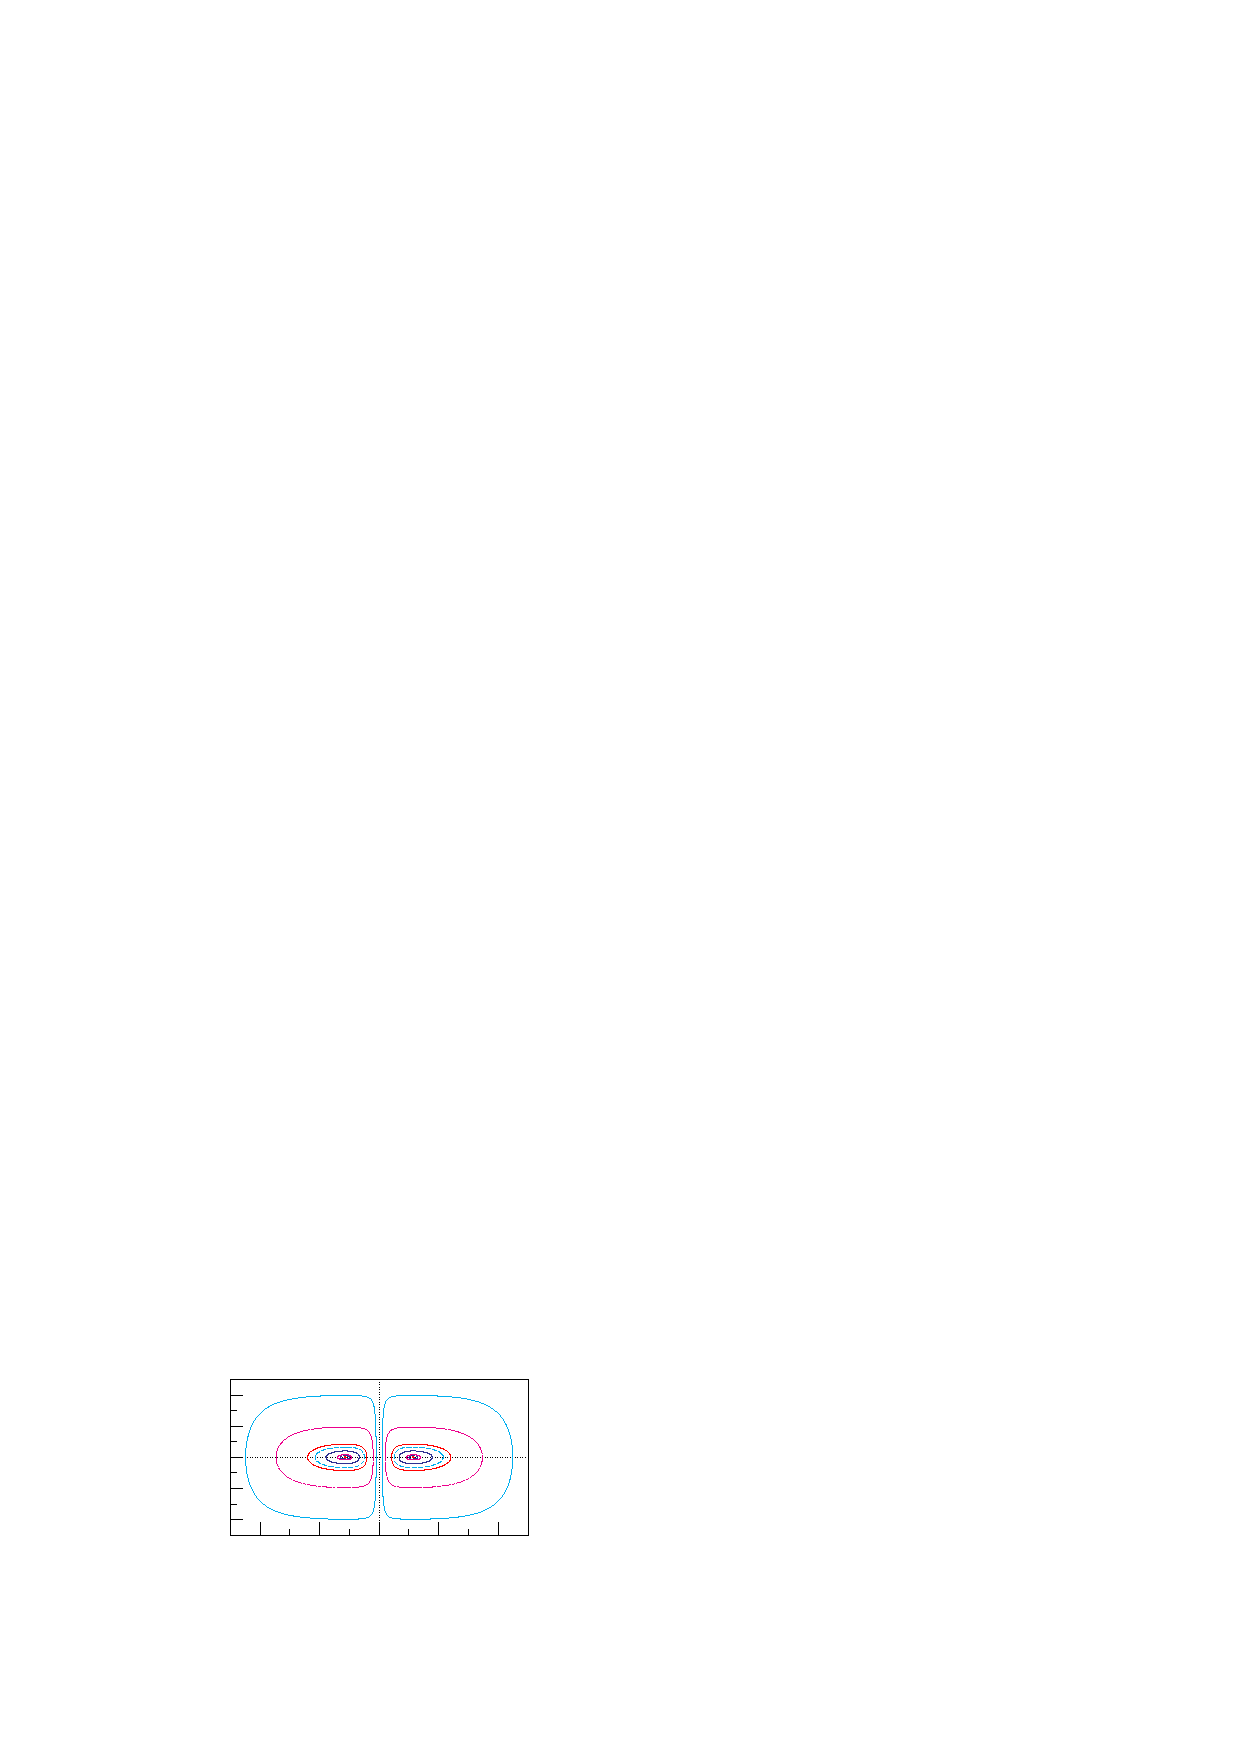
\includegraphics{Images/epslatex/nonaligned_phase}%
\end{picture}%
\begingroup
\setlength{\unitlength}{0.0200bp}%
\begin{picture}(9900,5940)(0,0)%
\put(1650,2024){\makebox(0,0)[r]{\strut{}-2}}%
\put(1650,2772){\makebox(0,0)[r]{\strut{}-1}}%
\put(1650,3520){\makebox(0,0)[r]{\strut{} 0}}%
\put(1650,4268){\makebox(0,0)[r]{\strut{} 1}}%
\put(1650,5016){\makebox(0,0)[r]{\strut{} 2}}%
\put(2640,1100){\makebox(0,0){\strut{}-2}}%
\put(4070,1100){\makebox(0,0){\strut{}-1}}%
\put(5500,1100){\makebox(0,0){\strut{} 0}}%
\put(6930,1100){\makebox(0,0){\strut{} 1}}%
\put(8360,1100){\makebox(0,0){\strut{} 2}}%
\put(550,3520){\rotatebox{90}{\makebox(0,0){\strut{}$p_{\theta}^{}$}}}%
\put(5500,275){\makebox(0,0){\strut{}$\theta$}}%
\end{picture}%
\endgroup
\endinput
 
\end{center}
\caption[Nonaligned equivalent oscillator]{\baselineskip=1.0\normalbaselineskip%
Phase diagram when $\alpha\ne\beta$. On the separatrix given by $\theta=0$ the aligned phase diagram is shown below. The uniform load parameter is $m=1.7$ and the energy levels are $h=3, \, 2, \, 1, \, 0.6$. Thus in both cases the separatrices delineate between classes of chirality.}
\label{fig:nonalignment}
\end{figure}
% 
\begin{figure}[!htbp]
\begin{center}
\input{Images/epslatex/elastica.tex} 
\end{center}
% \vspace*{-0.5cm}
\caption[Planar elastica]{\baselineskip=1.0\normalbaselineskip% 
Phase diagram when $\alpha=\beta=0$. The configurations are given by the load parameter $m=1.7$ and the energies $h=1, \, 0.8, \, 0.6, \, 0.4, \, 0.346, \, 0.2, \, 0,  \, -0.2$}
\label{fig:planar}
\end{figure}
%
\begin{figure}[h!tbp]
\begin{center}
\subfigure[][]{ \input{Images/epslatex/kov_n1.tex} \label{fig:kov_n1} }
\subfigure[][]{ \input{Images/epslatex/kov_n2.tex} \label{fig:kov_n2} }
\subfigure[][]{ %GNUPLOT: LaTeX picture with Postscript
\begin{picture}(0,0)%
\includegraphics{Images/epslatex/kov_n3}%
\end{picture}%
\begingroup
\setlength{\unitlength}{0.0200bp}%
\begin{picture}(9900,6480)(0,0)%
\put(2200,1650){\makebox(0,0)[r]{\strut{}-0.2}}%
\put(2200,2363){\makebox(0,0)[r]{\strut{} 0}}%
\put(2200,3077){\makebox(0,0)[r]{\strut{} 0.2}}%
\put(2200,3790){\makebox(0,0)[r]{\strut{} 0.4}}%
\put(2200,4503){\makebox(0,0)[r]{\strut{} 0.6}}%
\put(2200,5217){\makebox(0,0)[r]{\strut{} 0.8}}%
\put(2200,5930){\makebox(0,0)[r]{\strut{} 1}}%
\put(2475,1100){\makebox(0,0){\strut{} 0}}%
\put(4125,1100){\makebox(0,0){\strut{} 0.5}}%
\put(5775,1100){\makebox(0,0){\strut{} 1}}%
\put(7425,1100){\makebox(0,0){\strut{} 1.5}}%
\put(9075,1100){\makebox(0,0){\strut{} 2}}%
\put(550,3790){\rotatebox{90}{\makebox(0,0){\strut{}$n_{3}$}}}%
\put(5775,275){\makebox(0,0){\strut{}$s$}}%
\end{picture}%
\endgroup
\endinput
 \label{fig:kov_n3} }
\subfigure[][]{ \input{Images/epslatex/kov_m1.tex} \label{fig:kov_m1} }
\subfigure[][]{ \input{Images/epslatex/kov_m2.tex} \label{fig:kov_m2} }
\subfigure[][]{ \input{Images/epslatex/kov_m3.tex} \label{fig:kov_m3} }
\end{center}
\caption[Force and moments of Lagrange and Kovalevskaya homoclinics]{\baselineskip=1.0\normalbaselineskip%
Force and moments of Lagrange (blue) and Kovalevskaya (red) homoclinics when $m=1.70$. The forces and moments were found numerically using a shooting method. Details of the shooting method can be found in the appendix~\ref{chap:numerics}.}
\label{fig:kov}
\end{figure} % 
%
% \section{Action-Angle Formulation} \label{sec:action_angle}
% %
% The Arnol'd-Liouville theorem requires that the level sets be compact for an action-angle formulation, and as has been mentioned this is not the case. Thus in this section, from~\cite{Kehrbaum97a,Arnold89} local action-angle are created and solutions classified from the nature of the action-angle formulation on the $3$-torus. 
% %
% \par
% In order for the Hamilton-Jacobi equation to be separable it is necessary to apply the end force about the $\boldsymbol{d}_{3}$ axis as this director is independent of the angle $\phi$. Thus the system is a single degree of freedom problem. To convert the Hamiltonian from Euler angles into action-angles a generating function $S\left(\theta, I\right)$ which is a solution to the Hamilton-Jacobi equation is introduced
% %
% \begin{align}
% \frac{1}{2}\left( \frac{\partial S}{\partial \theta}\right)^{2} + \frac{1}{2}\left( \frac{ \frac{\partial S}{\partial \psi} - \frac{\partial S}{\partial \phi}\cos\theta }{\sin\theta} \right)^{2} + \frac{\cos\theta}{m^{2}} & = h. \label{eq:general_generating_function}
% \end{align}
% %
% The generating function is then used to find the actions and then the angles
% %
% \begin{equation}
% I_{i} = \frac{1}{2\pi} \oint \frac{\partial S}{\partial q_{i}} \mathrm{d}q_{i}, \quad \mbox{and} \quad \varphi_{i} = \frac{\partial S}{\partial I_{i}} \nonumber 
% \end{equation}
% %
% where the integrals are taken over one cycle of the torus. In order to decouple the actions, the function $S$ is decomposed into three parts
% %
% \begin{align}
% S &= S_{1}\left( I_{1},I_{2},I_{3}, \theta\right) + I_{2} \phi + I_{3}\psi, \nonumber
% \end{align} 
% %
% where the first part is determined by
% %
% \begin{align}
% \frac{\partial S_{1}}{\partial \theta} & = \sqrt{ 2h - \left(\frac{ I_{3} - I_{2} \cos\theta}{\sin^{2}\theta}\right)^{2} - \frac{2\cos\theta}{m^{2}} }. \nonumber
% \end{align}
% %
% Hence, from the substitution $u=\cos\theta$ the nontrivial part of the generating function is given by   
% %
% \begin{align}
% S_{1} & = \int_{u_{1}}^{u} \frac{\sqrt{f\left(u\right) } }{ 1 - u^{2} } \mathrm{d}u, \quad \mbox{where} \quad f\left(u\right) = 2\left(h-u\slash m^{2}\right)\left(1-u^{2}\right) - \left( I_{3} - I_{2} u \right)^{2}, \nonumber
% \end{align}
% %
% where it is assumed that the polynomial $f\left(u\right)$ has three not necessarily unique real roots which satisfy $ -1 < u_{1} \le u_{2} < 1 < u_{3}$. Thus 
% %
% \begin{align}
% f\left(u\right) & = \frac{1}{m^{2}}\left(u-u_{1}\right)\left(u-u_{2}\right)\left(u-u_{3}\right). \nonumber 
% \end{align}
% %
% The actions are given by
% %
% \begin{subequations}
% \begin{align}
% I_{1} & = \frac{1}{\pi} \int_{u_{1}}^{u_{2}} \frac{\sqrt{f\left(u\right) } }{ 1 - u^{2} } \mathrm{d}u, \nonumber \\
% I_{2} & = p_{\psi}, \nonumber \\
% I_{3} & = p_{\phi}, \nonumber 
% \end{align}
% \end{subequations}
% %
% where $I_{1}$ is expressed implicitly as $I_{1} = \tilde{I}_{1}\left(I_{2},I_{3},h\right)$ which in turn allows $h=\tilde{\mathcal{H}}\left(I_{1},I_{2},I_{3}\right)$ to be expressed implicitly. Hence, without loss of generality  $I_{1} = \tilde{I}_{1}\left(I_{2},I_{3},\tilde{\mathcal{H}}\left(I_{1},I_{2},I_{3}\right)\right)$. Thus substituting this expression into the nontrivial part of the generating function yields $S_{1}\left(\theta, I_{1}, I_{2}, I_{3}\right)= \tilde{S}_{1}\left(\theta, I_{2},I_{3}, \tilde{\mathcal{H}}\left(I_{1},I_{2},I_{3}\right)\right) = \tilde{S}_{1}\left(\theta, I_{2},I_{3}, h\right)$. Hence the angles are given by
% %
% \begin{subequations}
% \begin{align}
% \varphi_{1} & = \frac{\partial S}{\partial I_{1} } = \frac{\partial \tilde{S}_{1}}{\partial h} \frac{\partial \tilde{\mathcal{H}}}{\partial I_{1}} = \frac{\partial \tilde{S}_{1}}{\partial h}\omega_{1}, \\ 
% \varphi_{2} & = \frac{\partial S}{\partial I_{2} } = \phi + \frac{\partial S_{1} }{\partial I_{2} } = \phi + \frac{\partial \tilde{S}_{1} }{\partial I_{2} } + \frac{\partial \tilde{S}_{1}}{\partial h} \frac{\partial \tilde{\mathcal{H}} }{\partial I_{2}} = \phi + \frac{\partial \tilde{S}_{1} }{\partial I_{2} } + \frac{\partial \tilde{S}_{1}}{\partial h} \omega_{2}, \\
% \varphi_{3} & = \frac{\partial S}{\partial I_{3} } = \psi + \frac{\partial S_{1} }{\partial I_{3} } = \psi + \frac{\partial \tilde{S}_{1} }{\partial I_{3} } + \frac{\partial \tilde{S}_{1}}{\partial h} \frac{\partial \tilde{\mathcal{H}} }{\partial I_{3}} = \psi + \frac{\partial \tilde{S}_{1} }{\partial I_{3} } + \frac{\partial \tilde{S}_{1}}{\partial h} \omega_{3}.
% \end{align}
% \end{subequations}
% %
% where
% %
% \begin{align}
% \omega_{i} & = \dfrac{\partial \tilde{\mathcal{H}}}{\partial I_{i}}. \nonumber
% \end{align}
% %
% Then, by implicitly differentiation
% %
% \begin{subequations}
% \begin{align}
% \omega_{1} & = \dfrac{\partial \tilde{\mathcal{H}}}{\partial I_{1}} = \left( \dfrac{\partial \tilde{I}_{1}}{\partial h}\right)^{-1}, \\
% \omega_{2} & = \dfrac{\partial \tilde{\mathcal{H}}}{\partial I_{2}} =-\left( \dfrac{\partial \tilde{I}_{1}}{\partial h}\right)^{-1} \dfrac{\partial \tilde{I}_{1}}{\partial I_{2}}, \\
% \omega_{3} & = \dfrac{\partial \tilde{\mathcal{H}}}{\partial I_{3}} =-\left( \dfrac{\partial \tilde{I}_{1}}{\partial h}\right)^{-1} \dfrac{\partial \tilde{I}_{1}}{\partial I_{3}}. 
% \end{align}
% \end{subequations}
% %
% Thus by the definition of the elliptic integrals the frequencies are
% %
% \begin{subequations}
% \begin{align}
% \omega_{1} & = \frac{\pi}{2} m \sqrt{ u_{3} - u_{1} } \frac{1}{K}, \\
% \omega_{2} & = \frac{1}{K} Q_{+}\left(\frac{\pi}{2}\right), \\
% \omega_{3} & = \nu I_{3} - \frac{1}{2K}Q_{-}\left(\frac{\pi}{2}\right)
% \end{align}
% \end{subequations}
% %
% and the angles given by
% %
% \begin{subequations}
% \begin{align}
% \varphi_{1} & = \dfrac{\pi}{K} F\left(v,\sqrt{\dfrac{u_{2}-u_{1}}{u_{3}-u_{1}}}\right), \\
% \varphi_{2} & = \psi + \dfrac{m}{ \sqrt{u_{3}-u_{1}} K} \left( Q_{-}\left(v\right)K - Q_{-}\left(\dfrac{\pi}{2}\right) F\left(v,\sqrt{\dfrac{u_{2}-u_{1}}{u_{3}-u_{1}}} \right) \right), \\
% \varphi_{3} & = \phi - \dfrac{m}{ \sqrt{u_{3}-u_{1}} K} \left( Q_{+}\left(v\right)K - Q_{+}\left(\dfrac{\pi}{2}\right) F\left(v,\sqrt{\dfrac{u_{2}-u_{1}}{u_{3}-u_{1}}} \right) \right)
% \end{align}
% \end{subequations}
% %
% where
% %
% \begin{align}
% Q_{\pm}\left(v\right) & = \dfrac{I_{2}-I_{3}}{1-u_{1}} \Pi \left( v, \dfrac{u_{2}-u_{1}}{1-u_{1}}, \sqrt{ \dfrac{u_{2}-u_{1}}{u_{3}-u_{1}} } \right) \pm  \dfrac{I_{2}+I_{3}}{1+u_{1}}\Pi \left( v, -\dfrac{u_{2}-u_{1}}{1+u_{1}}, \sqrt{ \dfrac{u_{2}-u_{1}}{u_{3}-u_{1}} } \right). \nonumber
% \end{align}
%
% \subsection{Hamiltonian-Hopf Bifurcation}
% %
% Of interest are homoclinic solutions which only occur when $p_{\psi}=p_{\phi}=1$ and $h=1\slash{m^{2}}$. Thus for homoclinic solutions the generating function is given by
% %
% \begin{align}
% S & = S_{1}\left(I_{1},I_{2},I_{3},\theta\right) + \psi I_{2} + \phi I_{3}, \nonumber
% \end{align}
% %
% In contrast to general case~\eqref{eq:general_generating_function} specifying $p_{\psi}=p_{\phi}=1$ then gives have a single root at $u=1$ and two nontrivial roots, 
% %
% \begin{align}
% S_{1} & = \dfrac{2}{m} \int_{?}^{u} \dfrac{ \sqrt{f\left(u\right)} }{ 1 - u^{2} } \, \mathrm{d}s \quad \mbox{where} \quad f\left(u\right) = \left(1-u\right)\left( 2\left(h-u\slash m^{2}\right) - \left(1-u\right)\right). \nonumber
% \end{align}
% %
% However if the energy is set as the homoclinic energy $h=1\slash{m^{2}}$ the polynomial has one nontrivial root and a double root at $u=1$ and the root of the polynomial is simply $u_{1} = u_{0}$. 
% %
% \begin{align}
% S_{1} & = \dfrac{2}{m} \int_{?}^{u} \dfrac{ \sqrt{f\left(u\right)} }{ 1 + u } \, \mathrm{d}s \quad \mbox{where} \quad f\left(u\right) = u - u_{0} \quad \mbox{and} \quad u_{0} = m^{2}\slash 2 - 1. \nonumber
% \end{align}
% %
% The angles are given by
% %
% \begin{subequations}
% \begin{align}
% I_{1} & = \dfrac{1}{\pi m} \int_{ u_{0} }^{1} \dfrac{ u - u_{0} }{ 1 + u } \, \mathrm{d}s = \dfrac{2}{\pi}\sqrt{1-u_{0}}\left( 1 - \tan^{-1}\left(\sqrt{\dfrac{1-u_{0}}{1+u_{0}}}\right) \right) \\
% I_{2} & = p_{\phi}, \\
% I_{3} & = p_{\psi}. 
% \end{align}
% \end{subequations}
% %
% Thus the frequencies of the angle coordinates are given by
% %
% \begin{subequations}
% \begin{align}
% \omega_{1} & = \int_{ u_{0} }^{1} \dfrac{2}{\sqrt{2h\left(1+u\right)-1}}\,\mathrm{d}u = 2\sqrt{1-u_{0}}, \\
% \omega_{2} & = b, \\
% \omega_{3} & = b. 
% \end{align}
% \end{subequations}
% %
% and the angles 
% %
% \begin{subequations}
% \begin{align}
% \varphi_{1} & = b, \\
% \varphi_{2} & = b, \\
% \varphi_{3} & = b. 
% \end{align}
% \end{subequations}
% %
% Hence as $m\rightarrow2$ then the actions $I_{1}$ and $I_{2}$ becomes ill-defined since $u_{0} \rightarrow 0$. \textbf{Thus the system reduces from a three-tori to a one-torus, from a completely integrable system, to a maximally superintegrable system, at the bifurcation point.} 
% %
% \subsection{The Elastica}
% %
% With $p_{\psi}=p_{\phi}=0$ the elastica simply reduces down to 
% %
% \begin{align}
% S & = 4 \sqrt{2} \int_{u_{0}}^{u}  \dfrac{ \sqrt{h-u\slash{m^{2}}} }{1-u^{2}} \, \mathrm{d}u, \quad \mbox{where} \quad u_{0} = hm^2, \nonumber
% \end{align}
% %
% hence the action is 
% %
% \begin{align}
% I & = \dfrac{1}{\pi} \int_{-1}^{ h m^{2} }  \dfrac{ \sqrt{h-u\slash{m^{2}}} }{1-u^{2}} \, \mathrm{d}u , \nonumber\\
% & = \nonumber
% \end{align}
% %
% and the angle is
% %
% \begin{align}
% \varphi & =  \dfrac{\partial S}{\partial I} \nonumber \\
% & = \dfrac{\partial S}{\partial h} \dfrac{\partial h}{\partial I} \nonumber \\
% & = \nonumber
% \end{align}
% %
% Thus as there is no topological change in the tori a bifurcation never occurs for any value of the load parameter.
%
\subsection{Extensibility} \label{subsec:integrable_perturbations}
%
It has been shown by finding explicit solutions without exploiting the Hamiltonian structure, that if an isotropic rod is shearable and extensible then it remains integrable~\cite{Stump00}. In this section, by exploiting the Hamiltonian structure closed form expressions for homoclinic solutions are derived.
%
\par
In the case of isotropic bending $\left(\rho=0\right)$, shear and extension $\left(\sigma=0\right)$ the governing equation can be reduced to a single degree of freedom Hamiltonian system by substituting the moments~\eqref{eq:noncanonical_moment1} and forces~\eqref{eq:kirchhoff_canonical_force} into the Hamiltonian
%
\begin{align}
\mathcal{H} & = \dfrac{1}{2}m_{1}^{2}+\dfrac{1}{2}m_{2}^{2}+\dfrac{1}{2}\left(1+\nu\right)m_{1}^{2} + \dfrac{1}{2m^{2}}\epsilon n_{1}^{2} + \dfrac{1}{2m^{2}}\epsilon n_{2}^{2} + \dfrac{1}{2m^{2}}\epsilon\left(1+\gamma\right)n_{3}^{2} + \dfrac{n_{3}}{m^{2}}. 
\end{align}
%
The Hamiltonian is given by
%
\begin{align}
\mathcal{H}\left( \theta, p_{\theta} \right) & = \frac{1}{2} p_{\theta}^{2} + \frac{1}{2} \left( \frac{p_{\psi}-p_{\phi}\cos\theta}{\sin\theta} \right)^{2} + \frac{1}{2}\left(1+\nu\right)p_{\phi}^{2} + \frac{\cos\theta\left( \epsilon\gamma\cos\theta + 2 \right)}{2m^{2}} + \frac{\epsilon}{2m^{2}} \label{eq:extensible_ham}.
\end{align}
%
The additional constant term $\epsilon \slash 2m^{2}$ is stored energy due to shearability. Thus, when $\alpha=\beta=1$, Hamilton's equations are given by
%
\begin{subequations}
\begin{align}
{\theta}^{\prime} & = p_{\theta}, \\
{p}_{\theta}^{\prime} & = \frac{\sin\theta}{\left(1+\cos\theta\right)^{2}} - \frac{\left(\epsilon\gamma\cos\theta+1\right)\sin\theta}{m^{2}}.
\end{align}
\end{subequations}
%
Solving for fixed points yields the trivial solution $p_{\theta}=0$ and $\sin\theta = 0$ and the nontrivial fixed points
%
\begin{align} 
0 & = \frac{1}{\left(1+\cos\theta\right)^{2}} - \frac{\epsilon\gamma\cos\theta+1}{m^{2}}.
\end{align}
%
Thus, the real solutions to the cubic
%
\begin{align}
0 & = \epsilon \gamma \cos^{3}\theta + \cos^{2}\theta + \epsilon \gamma \cos\theta + 1-m^{2}
\end{align}
%
determine the configurations for helices and hence the buckling load. It should be noted that only a single helix exists when $\epsilon\gamma$ is small since solutions to the equation are required to be real-valued angles and the equation has two imaginary roots and a single real root. The condition for three real roots is given by
%
\begin{align}
\left(1-\dfrac{1}{3}\dfrac{1}{\epsilon\gamma}\right)^{3}\slash{27} + \left(\dfrac{1}{\epsilon\gamma}\right)^{2}\left(\dfrac{2}{27}\left(\dfrac{1}{\epsilon\gamma}\right)^{2} + \dfrac{2}{3} -m^{2} \right)^{2}\slash{4} \ge 0
\end{align}
%
% Substituting the real root of the cubic into the formula for a helix yields the buckling value for the extensible rod. 
Previously the analysis of the buckling of an extensible rod had been derived by linearisation~\cite{Champneys97b}. 
%
\par
Nontrivial solutions can be found from the integral
%
\begin{align}
s & = \int_{u\left(0\right)}^{u\left(s\right)} \dfrac{\mathrm{d}u}{ \sqrt{2\left( h-u\left(u \epsilon\gamma\slash 2 +1\right)\slash m^{2}\right)\left(1-u^{2}\right)-\left(\alpha-\beta u\right)^{2} } }.
\end{align}
%
The homoclinic now has energy given by 
%
\begin{align}
h & = \dfrac{1}{m^{2}}\left(1+\dfrac{\epsilon\gamma}{2}\right) \nonumber
\end{align}
%
which, along with the torque condition $\alpha=\beta=1$ yields the integral
%
\begin{align}
s & = \int_{u\left(0\right)}^{u\left(s\right)} \dfrac{\mathrm{d}u}{ \left(1-u\right)\sqrt{ \epsilon\gamma \left(u+1\right)^{2} \slash m^{2} + 2\left(u+1\right)\slash m^{2} + 1 } }. \nonumber
\end{align}
%
The integral can be expressed in the form
%
\begin{align}
s & = \dfrac{m}{\sqrt{\epsilon\gamma}} \int_{u\left(0\right)}^{u\left(s\right)} \dfrac{ \mathrm{d}u }{ \left(1-u\right) \sqrt{ f\left(u\right) } }, \quad \mbox{where} \quad f\left(u\right) = u^{2} + 2 u\left(1+\dfrac{1}{\epsilon\gamma}\right) + 1 + \dfrac{2}{\epsilon\gamma} -\dfrac{m^{2}}{\epsilon\gamma}. \nonumber
\end{align}
%
The quadratic $f\left(u\right)$ has roots
%
\begin{align}
u_{\pm} & = -\left(1+\dfrac{1}{\epsilon\gamma}\right) \pm \dfrac{1}{\epsilon\gamma}\sqrt{ 1 + \epsilon \gamma m^{2} }, \nonumber
\end{align}
%
which in the limit of small extensibility, that is $\epsilon \gamma m^{2} \ll 1$, yields
%
\begin{align}
u_{+} & = \dfrac{m^{2}}{2} - 1 - \dfrac{1}{8}\left( \epsilon\gamma m^{2} \right)^{2} + \frac{1}{16}\left( \epsilon\gamma m^{2} \right)^{3} + \mathcal{O}\left(\epsilon^{4}\right), \nonumber \\ 
u_{-} & = -1 - \dfrac{m^{2}}{2} - \dfrac{2}{\epsilon\gamma} + \dfrac{1}{8}\left( \epsilon\gamma m^{2} \right)^{2} - \frac{1}{16}\left( \epsilon\gamma m^{2} \right)^{3} + \mathcal{O}\left(\epsilon^{4}\right). \nonumber 
\end{align}
%
So that the roots scale as perturbations of the inextensible rod, that is $u_{+} \sim u_{0}$ and $u_{-} \sim -1$. Hence the limits of integration become
%
\begin{align}
s & = \dfrac{m}{\sqrt{\epsilon\gamma}}\int_{u_{+}}^{u\left(s\right)}\dfrac{\mathrm{d}z}{\left(1-u\right)\sqrt{\left(u+u_{-}\right)\left( u-u_{+}\right)}}. \nonumber
\end{align}
%
On the substitution $u = -u_{-} + \left(u_{-}+u_{+}\right)\cosh^{2} z $ the integral becomes
%
\begin{align}
s & = \dfrac{2m}{\left(1+u_{-}\right)\sqrt{\epsilon\gamma}} \int_{0}^{z\left(s\right)} \dfrac{ \mathrm{d}z }{ 1 - k \cosh^{2}z } , \quad \mbox{with} \quad k = \dfrac{u_{-}+u_{+}}{1+u_{-}},
\end{align}
%
where
%
\begin{align}
z\left(s\right) & = \cosh^{-1} \sqrt{ \dfrac{u\left(s\right)-u_{-}}{u_{+}+u_{-}} } \nonumber
\end{align}
%
and the integral is given by
%
\begin{align}
\int \dfrac{\mathrm{d}z}{1 - k \cosh^{2} z} & = \dfrac{-2}{\sqrt{k^{2}-1}} \tan^{-1}\left( \sqrt{\dfrac{k+1}{k-1}}\tanh \dfrac{z}{2} \right).  \label{eq:ext_homoclinic}
\end{align}
%
In the limit of $\epsilon \rightarrow 0$ the Kirchhoff homoclinic~\eqref{eq:isotropic_homoclinic} is recovered. The derivative of the angle $\psi$ is given by
%
\begin{align}
{\psi}^{\prime} & = \frac{1}{1+\cos\theta}. \label{eq:extensibility_psi}
\end{align} 
%
\par
The evolutions of the Euler angles and their conjugtaes are quantatively the same as those displayed in figures~\ref{fig:evolutions} and~\ref{fig:omegas} and so are not presented.
% 
\section{Nonintegrable Perturbations} \label{sec:nonintegrable_perturbations}
%
In this section anisotropy and initial curvature~\cite{Heijden98a,Champneys97a} are shown to destroy integrability.
%
\par
For material perturbations the constitutive relations change but the force and moment balance remain the same. Thus, the Casimirs remain the same, and hence the reduction holds.  Both cases have been studied before but in a different formulation using Deprit variables.
%
\par
The Hamiltonian system now takes the general form
%
\begin{align}
\mathcal{H}_{\epsilon}\left(\theta,\phi,p_{\theta},p_{\phi},p_{\psi}\right) & = \mathcal{H}_{0}\left(\theta,p_{\theta},p_{\phi},p_{\psi}\right) + \epsilon \mathcal{H}_{1}\left(\theta,\phi,p_{\theta},p_{\phi},p_{\psi}\right),
\end{align} 
%.
where the unperturbed Hamiltonian is given by~\eqref{eq:two_dim_ham}, the unperturbed homoclinic by~\eqref{eq:isotropic_homoclinic} and the frequency of the angle $\phi$ is given by

\begin{align}
\omega_{0} & = \dfrac{\partial \mathcal{H}_{0}}{\partial p_{\phi}} = \nu + \dfrac{2}{m^{2} + \left(4+m^{2}\right)\tanh^{2}\left(\dfrac{\sqrt{4+m^{2}}}{2m}s\right)}. \label{eq:Omega_0_explicit}
\end{align}
%
Thus when $\nu\ge0$ then $\omega_{0} \ge \delta > 0$ for a small, fixed $\delta$. The equilibrium point~\eqref{eq:trivial_fp} from which the homoclinic eminates from is a hyperbolic saddle. Thus Mel'nikov's method, as described in \S\ref{sec:melnikov_thm}, may be applied to test for the breakup of integrability due to the loss of the Lagrange integral $p_{\phi}$.
%
% \par
% It should be noted that the canonical system is still invariant under the action of $S^{1}$, thus the modified version of Mel'nikov's method, as described in, is required. Note that in all cases considered in this section the system is perturbed by a single term of order $\epsilon$. The Mel'nikov analysis still only provides a first order approximation to the rate of splitting of the unstable and stable manifolds, as the action-angle variables can still expressed as a series in the perturbation parameters.
%
\par
The partial derivatives of the unperturbed Hamiltonian and angular frequency evaluated at the homoclinic energy level are given by
%
\begin{subequations}
\label{eq:partials}
\begin{align}
\dfrac{\partial \mathcal{H}_{0}}{\partial \theta} & = \dfrac{\sin\theta}{\left(1+\cos\theta\right)^{2}} - \dfrac{\sin\theta}{m^{2}}, \\
\dfrac{\partial \mathcal{H}_{0}}{\partial p_{\theta}} & = p_{\theta}, \\
\dfrac{\partial \omega_{0}}{\partial \theta} & = \dfrac{\sin\theta}{\left(1+\cos\theta\right)^{2}}, \\
\dfrac{\partial \omega_{0}}{\partial p_{\theta}} & = 0 .
\end{align}
\end{subequations}
%
That $p_\theta$ is an odd function and $\theta$ and $\omega_{0}$ are even functions will be used to simplify the Mel'nikov integral.
% 
\subsection{Anisotropy} \label{subsec:anisotropy}
%
When the rod is linearly elastic, unshearable, inextensible, initially straight and anisotropic the constitutive relations are given by
%
\begin{align}
\mathcal{W}\left(\mathsf{u}\right) & = \frac{1}{2} B_{1} u_{1}^{2} + \frac{1}{2} B_{2} u_{1}^{2} + \frac{1}{2} C u_{3}^{2}. 
\end{align}
%
The nondimensional Hamiltonian is given by
%
\begin{align}
\mathcal{H} & = \frac{1}{2}p_{\theta}^{2} +  \left(\frac{p_{\psi}-p_{\phi}\cos\theta}{\sin\theta}\right)^{2} + \frac{1}{2}\left(1+\nu\right)p_{\phi}^{2} + \frac{\cos\theta}{m^{2}} \nonumber \\ 
& \hspace{3.0cm} + \frac{\rho}{2} \left( p_{\theta}\sin\phi - \cos\phi\left(\frac{p_{\psi}-p_{\phi}\cos\theta}{\sin\theta}\right) \right)^{2}.
\end{align}
%
Hamilton's equations are
%
\begin{subequations}
\label{eq:dot}
\begin{align}
{\theta}^{\prime} & = p_{\theta} + \rho\sin\phi\left( p_{\theta}\sin\phi - \cos\phi \left( \frac{p_{\psi}-p_{\phi}\cos\theta}{\sin\theta} \right) \right), \label{eq:dot_theta} \\
{\phi}^{\prime} & = \left(1+\nu\right) p_{\phi} - \cos\theta\left( \frac{p_{\psi}-p_{\phi}\cos\theta}{\sin^{2}\theta} \right) \nonumber \\
& \hspace{1.5cm} + \rho\frac{\cos\phi\cos\theta}{\sin\theta}\left( p_{\theta}\sin\phi - \cos\phi\left( \frac{p_{\psi}-p_{\phi}\cos\theta}{\sin\theta} \right) \right), \label{eq:dot_phi} \\
{\psi}^{\prime} & = \left(\frac{p_{\psi}-p_{\phi}\cos\theta}{\sin^{2}\theta}\right) - \rho\frac{\cos\phi}{\sin\theta}\left( p_{\theta}\sin\phi - \cos\phi\left(\frac{p_{\psi}-p_{\phi}\cos\theta}{\sin\theta}\right) \right), \label{eq:dot_psi}\\
{p}_{\theta}^{\prime} & = \frac{ \sin\theta }{ m^{2} } - \left( \frac{p_{\phi}-p_{\psi}\cos\theta}{\sin\theta} \right)\left( \frac{p_{\psi}-p_{\phi}\cos\theta}{\sin^{2}\theta} \right)\nonumber \\
& \hspace{1.5cm}- \rho\cos\phi\left( \frac{p_{\psi}-p_{\phi}\cos\theta}{\sin^{2}\theta} \right)\left( p_{\theta}\sin\phi - \cos\phi\left(\frac{p_{\phi}-p_{\psi}\cos\theta}{\sin\theta}\right)\right), \label{eq:dot_p_theta} \\  
{p}_{\phi}^{\prime} & = \rho\left(p_{\theta}\cos\phi+\sin\phi\left(\frac{p_{\phi}-p_{\psi}\cos\theta}{\sin\theta}\right) \right)\left(p_{\theta}\sin\phi - \cos\phi\left(\frac{p_{\phi}-p_{\psi}\cos\theta}{\sin\theta}\right)\right),\label{eq:dot_p_phi} \\
{p}_{\psi}^{\prime} & = 0. \label{eq:dot_p_psi}
\end{align}
\end{subequations}
%
Thus the six-dimensional noncanonical system~\eqref{eq:kirchhoff} is reduced to a four-dimensional canonical Hamiltonian system. Expressing $\phi\left(s\right) = \bar\phi\left(s\right)+\phi_{0}$ the perturbation to the Hamiltonian is of the form
%
\begin{align}
\mathcal{H}_{1} & = \dfrac{1}{2}\cos2\phi_{0} \left( \cos2\bar{\phi} \left(p_{\theta}^{2}+ \dfrac{1-\cos\theta}{1+\cos\theta}\right) - p_{\theta}\sin2\bar{\phi}\left(\dfrac{1-\cos\theta}{\sin\theta}\right)\right)  \nonumber \\
& \hspace{1.0cm} - \dfrac{1}{2}\sin2\phi_{0} \left( \sin2\bar{\phi} \left(p_{\theta}^{2} + \dfrac{1-\cos\theta}{1+\cos\theta}\right) + p_{\theta}\cos2\bar{\phi}\left(\dfrac{1-\cos\theta}{\sin\theta}\right)\right) \nonumber \\
& \hspace{2.0cm} - \dfrac{1}{2}p_{\theta}^{2} + \dfrac{1}{2}\left(\dfrac{1-\cos\theta}{1+\cos\theta}\right).
\end{align}
%
The partial derivatives of the perturbation are given by
%
\begin{subequations}
\label{eq:H1_partial_anisotropic}
\begin{align}
\dfrac{\partial \mathcal{H}_{1}}{\partial \theta} & = \dfrac{1}{2}p_{\theta}\left(\cos2\phi_{0}\cos2\bar{\phi} - \sin2\phi_{0}\sin2\bar{\phi}-1\right)\nonumber \\
& \hspace{1.0cm} + \left(1-\dfrac{1}{2}\left(\cos2\phi_{0}\cos2\bar{\phi}-\sin2\phi_{0}\sin2\bar{\phi}\right)\right)\left(\dfrac{1-\cos\theta}{\left(1+\cos\theta\right)\sin\theta} \right), \\
\dfrac{\partial \mathcal{H}_{1}}{\partial p_{\theta}} & = \dfrac{1}{2} p_{\theta}\left(\cos2\phi_{0}\cos2\bar{\phi}-\sin2\phi_{0}\sin2\bar{\phi}-1\right) \nonumber \\
& \hspace{1.0cm} - \dfrac{1}{2}\left(\sin2\phi_{0}\cos2\bar{\phi}-\cos2\phi_{0}\sin2\bar{\phi}\right)\left( \dfrac{1-\cos\theta}{\sin\theta} \right).
\end{align}
\end{subequations}
%
Hence the Mel'nikov integral is given by
%
\begin{align}
\mathcal{M}_{h}\left(\phi_{0}\right) & = \sin\phi_{0}\int^{+\infty}_{-\infty} A\left(s\right)\,\mathrm{d}s + \cos\phi_{0}\int^{+\infty}_{-\infty} B\left(s\right)\,\mathrm{d}s + \int^{+\infty}_{-\infty} C\left(s\right)\,\mathrm{d}s
\end{align}
%
where
%
\begin{subequations}
\begin{align}
A\left(s\right) & = \dfrac{1}{2}\left( \dfrac{1+\cos\theta}{m^{2}} + \dfrac{1}{1+\cos\theta} +p_{\theta}^{2}\right)\left(p_{\theta}\sin\theta\sin2\bar\phi-\left(1-\cos\theta\right)\cos2\bar\phi\right) \nonumber \\
& \hspace{1.0cm} + \dfrac{1}{2}p_{\theta}^{2}\cos\theta\left( \cos2\bar\phi + \sin2\bar\phi\left(\dfrac{1-\cos\theta}{\sin\theta}\right) \right), \\
B\left(s\right) & = \dfrac{1}{2}\left( \dfrac{1+\cos\theta}{m^{2}} + \dfrac{1}{1+\cos\theta} +p_{\theta}^{2}\right)\left(p_{\theta}\sin\theta\cos2\bar\phi-\left(1-\cos\theta\right)\sin2\bar\phi\right) \nonumber \\
& \hspace{1.0cm} + \dfrac{1}{2}p_{\theta}^{2}\cos\theta\left( \sin2\bar\phi - \cos2\bar\phi\left(\dfrac{1-\cos\theta}{\sin\theta}\right) \right), \\
C\left(s\right) & = \dfrac{1}{2} p_{\theta} \left( \dfrac{1-\cos\theta}{\sin\theta} + \dfrac{1+\cos\theta}{m^{2}} + \dfrac{1}{1+\cos\theta} + p_{\theta}^{2} \right).
\end{align}
\end{subequations}
%
Then the condition for simple zeroes is given by 
%
\begin{align}
\left| \dfrac{c}{ \sqrt{ a^{2} + b^{2} } } \right| \le 1 
\end{align}
% 
where
% 
\begin{align}
a = \int_{-\infty}^{\infty}A\left(s\right)\,\mathrm{d}s, \quad b = \int_{-\infty}^{\infty}B\left(s\right)\,\mathrm{d}s \quad \mbox{and} \quad c = \int_{-\infty}^{\infty}C\left(s\right)\,\mathrm{d}s. \nonumber
\end{align}
%
The Mel'nikov integral is evaluated in figure~\ref{fig:Mel_aniso_1.75} for a variety of values for $m$. The curves show that generically the Mel'nikov integral has simple zeroes.
%
\begin{figure}[!htbp]
\begin{center}
%GNUPLOT: LaTeX picture with Postscript
\begin{picture}(0,0)%
\includegraphics{Images/epslatex/Mel_aniso_m.eps}%
\end{picture}%
\begingroup
\setlength{\unitlength}{0.0200bp}%
\begin{picture}(18000,6480)(0,0)%
\put(2200,1650){\makebox(0,0)[r]{\strut{}-2.5}}%
\put(2200,2078){\makebox(0,0)[r]{\strut{}-2}}%
\put(2200,2506){\makebox(0,0)[r]{\strut{}-1.5}}%
\put(2200,2934){\makebox(0,0)[r]{\strut{}-1}}%
\put(2200,3362){\makebox(0,0)[r]{\strut{}-0.5}}%
\put(2200,3790){\makebox(0,0)[r]{\strut{} 0}}%
\put(2200,4218){\makebox(0,0)[r]{\strut{} 0.5}}%
\put(2200,4646){\makebox(0,0)[r]{\strut{} 1}}%
\put(2200,5074){\makebox(0,0)[r]{\strut{} 1.5}}%
\put(2200,5502){\makebox(0,0)[r]{\strut{} 2}}%
\put(2200,5930){\makebox(0,0)[r]{\strut{} 2.5}}%
\put(17175,1100){\makebox(0,0){\strut{}$2\pi$}}%
\put(13500,1100){\makebox(0,0){\strut{}$3\pi\slash{2}$}}%
\put(9825,1100){\makebox(0,0){\strut{}$\pi$}}%
\put(6150,1100){\makebox(0,0){\strut{}${\pi}\slash{2}$}}%
\put(2475,1100){\makebox(0,0){\strut{}0}}%
\put(550,3790){\makebox(0,0){\strut{}\rotatebox{90}{$\mathcal{M}^{\left(1\right)}_{h}\left(\phi_{0}\right)$} }}%
\put(9825,275){\makebox(0,0){\strut{}$\phi_0$}}%
%
%\put(6500,2250){\makebox(0,0){\strut{} {\tiny $m=1.70$} }}%
%\put(9000,5250){\makebox(0,0){\strut{} {\tiny $m=1.80$} }}%
\end{picture}%
\endgroup
\endinput
 \label{fig:Mel_aniso_1.75} 
\end{center}
\caption[Anisotropic Mel'nikov integral]{Mel'nikov integral for anisotropic rod with $\nu=1\slash{3}$ and $m = 1.70$, $1.72$, $1.74$, $1.76$, $1.78$, $1.80$ at the homoclinic energy level.}
\end{figure}
% 
\subsection{Initial Curvature} \label{subsec:curvature}
%
For a rod with initial curvature the constitutive relationship take the form
%
\begin{align}
\mathcal{W}\left(\mathsf{u}\right) & = \frac{B_{1}}{2}u_{1}^{2}-u_{0}u_{1} + \frac{B_{1}}{2}u_{2}^{2} + \frac{C}{2}u_{3}^{2}.
\end{align} 
% 
In the initially curved case the nondimensionalised Hamiltonian is given by
%
\begin{align}
\mathcal{H} & = \frac{1}{2}p_{\theta}^{2} + \frac{1}{2}\left(1+\nu\right)p_{\phi}^{2} + \frac{1}{2}\left( \frac{ p_{\psi} - p_{\phi}\cos\theta }{\sin\theta}\right)^{2} + \frac{\cos\theta}{m^{2}} \nonumber \\ 
& \hspace{4.0cm} + \frac{1}{2}\kappa_{0} \left( p_{\theta}\sin\phi - \cos\phi \left( \frac{p_{\psi}-p_{\phi}\cos\theta}{\sin\theta} \right) \right). 
\end{align} 
%
It is interesting to observe that the perturbation for initial curvature is the square root of the perturbation for anisotropy. The governing equations are
%
\begin{subequations}
\label{eq:curv}
\begin{align}
{\theta}^{\prime} & = p_{\theta} + \kappa_{0}\sin\phi, \label{eq:curv_theta} \\
{\phi}^{\prime} & = \left(1+\nu\right) p_{\phi} - \cos\theta\left( \frac{p_{\psi}-p_{\phi}\cos\theta}{\sin^{2}\theta} \right) + \kappa_{0}\frac{\cos\theta\cos\phi}{\sin\theta}, \label{eq:curv_phi} \\
{\psi}^{\prime} & = \left(\frac{p_{\psi}-p_{\phi}\cos\theta}{\sin^{2}\theta}\right) - \kappa_{0}\frac{\cos\phi}{\sin\theta}, \label{eq:curv_psi} \\
{p}_{\theta}^{\prime} & = \frac{ \sin\theta }{ m^{2} } - \left( \frac{p_{\phi}-p_{\psi}\cos\theta}{\sin\theta} \right)\left( \frac{p_{\psi}-p_{\phi}\cos\theta}{\sin^{2}\theta} \right) - \kappa_{0}\cos\phi\left( \frac{p_{\phi}-p_{\psi}\cos\theta}{\sin^{2}\theta} \right), \label{eq:curv_p_theta} \\ 
{p}_{\phi}^{\prime} & = -\kappa_{0} \left( p_{\theta}\cos\phi + \sin\phi\left(\frac{p_{\psi}-p_{\phi}\cos\theta}{\sin\theta} \right)\right), \label{eq:curv_p_phi} \\
{p}_{\psi}^{\prime} & = 0. \label{eq:curv_p_psi} 
\end{align}
\end{subequations}
%
The perturbation to the Hamiltonian is given by
%
\begin{align}
\mathcal{H}_{1} & = \sin\phi_{0}\left( p_{\theta}\cos\bar\phi + \sin\bar{\phi}\left(\dfrac{1-\cos\theta}{\sin\theta}\right) \right) + \cos\phi_{0}\left( p_{\theta}\sin\bar\phi - \cos\bar{\phi}\left(\dfrac{1-\cos\theta}{\sin\theta}\right) \right). \nonumber 
\end{align}
%
The partial derivatives of the perturbation to the Hamiltonian are given by
%
\begin{subequations}
\label{eq:H1_partial_curved}
\begin{align}
\dfrac{\partial \mathcal{H}_{1}}{\partial \theta} & = \dfrac{\sin\phi_{0}\sin\bar{\phi}-\cos\phi_{0}\cos\bar{\phi}}{1+\cos\theta}, \\
\dfrac{\partial \mathcal{H}_{1}}{\partial p_{\theta}} & = \sin\phi_{0}\cos\bar{\phi} + \sin\bar{\phi}\cos\phi_{0}.
\end{align}
\end{subequations}
%
Hence, substituting the results~\eqref{eq:partials} and~\eqref{eq:H1_partial_curved} into the bracket~\eqref{eq:melnikov_bracket} and then substituting the homoclinic solutions~\eqref{eq:isotropic_homoclinic} into the resulting expression gives a Mel'nikov function of the form
%
\begin{align}
\mathcal{M}_{h}\left(\phi_{0}\right) & = \sin\phi_{0}\int^{+\infty}_{-\infty} A\left(s\right) \, \mathrm{d}s + \cos\phi_{0}\int^{+\infty}_{-\infty} B\left(s\right) \, \mathrm{d}s,
\end{align}
%
where
%
\begin{subequations}
\begin{align}
A\left(s\right) & = p_{\theta}\cos\theta\sin\bar\phi - \left( \dfrac{1+\cos\theta}{m^{2}} + \dfrac{1}{1+\cos\theta} + p_{\theta}^{2} \right)\sin\theta\cos\bar\phi \\
B\left(s\right) & = p_{\theta}\cos\theta\cos\bar\phi + \left( \dfrac{1+\cos\theta}{m^{2}} + \dfrac{1}{1+\cos\theta} + p_{\theta}^{2} \right)\sin\theta\sin\bar\phi
\end{align}
\end{subequations}
%
It follows from the reversibilities of the homoclinic solutions that the Mel'nikov function can be simplified over the half range 
%
\begin{align}
\mathcal{M}_{h}\left(\phi_{0}\right) & = 2\cos\phi_{0}\int^{+\infty}_{0}\sin\bar\phi\sin\theta\left(\dfrac{1+\cos\theta}{m^{2}} + \dfrac{1}{1+\cos\theta} + p_{\theta}^{2}\right) \, \mathrm{d}s \nonumber \\
& \hspace{1.5cm} + 2\sin\phi_{0}\int^{+\infty}_{0}p_{\theta}\cos\theta\sin\bar\phi \, \mathrm{d}s. 
\end{align}
%
\par
In contrast to the anisotropic case, there is no constant term in the Mel'nikov function, thus there are no bounds on the existence of transverse intersections of the stable and unstable manifolds. In figure~\ref{fig:poincare_curv} Poincar\'e sections which show the loss of integrability are presented. 
%
\par
The Poincar\'e sections were computed by fixing the integrals $p_{\psi}=1$ and placing the initial conditions were placed near the (unpertubed) saddle: $p_{\theta}=\theta=1\slash1000$ with $p_{\phi}=1$ and solving $\mathcal{H}\left(\theta,p_\theta,\phi,p_{\phi}\right)=h$ for $\phi$. The section itself was defined by $\cos\phi=0$.
%
\begin{figure}[h!tbp]
\label{fig:poincare_curv}
\begin{center}
\subfigure[][$\kappa_{0}=0.001$]{ \input{Images/epslatex/Poincare_kappa_0.001.tex} \label{fig:curv_poincare_0.001} }
\subfigure[][$\kappa_{0}=0.005$]{ \input{Images/epslatex/Poincare_kappa_0.005.tex} \label{fig:curv_poincare_0.005} }
\subfigure[][$\kappa_{0}=0.01$]{  %GNUPLOT: LaTeX picture with Postscript
\begin{picture}(0,0)%
\includegraphics{Images/epslatex/Poincare_kappa_0.01.eps}%
\end{picture}%
\begingroup
\setlength{\unitlength}{0.0200bp}%
\begin{picture}(9900,6480)(0,0)%
\put(2200,5502){\makebox(0,0)[r]{\strut{} 0.4}}%
\put(2200,4646){\makebox(0,0)[r]{\strut{} 0.2}}%
\put(2200,3790){\makebox(0,0)[r]{\strut{} 0}}%
\put(2200,2934){\makebox(0,0)[r]{\strut{}-0.2}}%
\put(2200,2078){\makebox(0,0)[r]{\strut{}-0.4}}%
\put(9075,1100){\makebox(0,0){\strut{} 1.6}}%
\put(8250,1100){\makebox(0,0){\strut{} 1.4}}%
\put(7425,1100){\makebox(0,0){\strut{} 1.2}}%
\put(6600,1100){\makebox(0,0){\strut{} 1}}%
\put(5775,1100){\makebox(0,0){\strut{} 0.8}}%
\put(4950,1100){\makebox(0,0){\strut{} 0.6}}%
\put(4125,1100){\makebox(0,0){\strut{} 0.4}}%
\put(3300,1100){\makebox(0,0){\strut{} 0.2}}%
\put(2475,1100){\makebox(0,0){\strut{} 0}}%
\put(550,3790){\rotatebox{90}{\makebox(0,0){\strut{}$p_{\theta}$}}}%
\put(5775,275){\makebox(0,0){\strut{}$\theta$}}%
\end{picture}%
\endgroup
\endinput
 \label{fig:curv_poincare_0.010} }
\subfigure[][$\kappa_{0}=0.015$]{ \input{Images/epslatex/Poincare_kappa_0.015.tex} \label{fig:curv_poincare_0.015} }
\subfigure[][$\kappa_{0}=0.02$]{  %GNUPLOT: LaTeX picture with Postscript
\begin{picture}(0,0)%
\includegraphics{Images/epslatex/Poincare_kappa_0.02.eps}%
\end{picture}%
\begingroup
\setlength{\unitlength}{0.0200bp}%
\begin{picture}(9900,6480)(0,0)%
\put(2200,2078){\makebox(0,0)[r]{\strut{}-0.4}}%
\put(2200,2934){\makebox(0,0)[r]{\strut{}-0.2}}%
\put(2200,3790){\makebox(0,0)[r]{\strut{} 0}}%
\put(2200,4646){\makebox(0,0)[r]{\strut{} 0.2}}%
\put(2200,5502){\makebox(0,0)[r]{\strut{} 0.4}}%
\put(2475,1100){\makebox(0,0){\strut{} 0}}%
\put(3355,1100){\makebox(0,0){\strut{} 0.2}}%
\put(4235,1100){\makebox(0,0){\strut{} 0.4}}%
\put(5115,1100){\makebox(0,0){\strut{} 0.6}}%
\put(5995,1100){\makebox(0,0){\strut{} 0.8}}%
\put(6875,1100){\makebox(0,0){\strut{} 1}}%
\put(7755,1100){\makebox(0,0){\strut{} 1.2}}%
\put(8635,1100){\makebox(0,0){\strut{} 1.4}}%
\put(550,3790){\rotatebox{90}{\makebox(0,0){\strut{}$p_{\theta}$}}}%
\put(5775,275){\makebox(0,0){\strut{}$\theta$}}%
\end{picture}%
\endgroup
\endinput
 \label{fig:curv_poincare_0.020} }
\subfigure[][$\kappa_{0}=0.05$]{  \input{Images/epslatex/Poincare_kappa_0.05.tex} \label{fig:curv_poincare_0.050} }
\end{center}
% \vspace*{-0.5cm}
\caption[Poincar\'e sections for initially curved rods on homoclinic energy level]{\baselineskip=1.0\normalbaselineskip%
Poincar\'e sections for initially curved rods on the unperturbed homoclinic energy level $h=1\slash m^{2}$ for varying levels of $\kappa_{0}$ on the hypersection determined by $\cos\phi=0$.}
\end{figure} % 
%
\section{Consequences of Nonintegrability} \label{sec:conseq} %
%
Mel'nikov analysis shows the existence of Smale horsehoes, which elegantly describe sensitivity to initial conditions. Arbitarily small changes in the perturbation $\mathcal{H}_{1}$ grow exponentially along the arclength until they reach the same order of magnitude as the field variables $\left(\mathsf{n},\mathsf{m}\right)$. A multiplicity of multimodal solutions now exists~\cite{Champneys96b}. But the system has a well defined bifurcation structure determined by acculumation and coalescence rules~\cite{Heijden98a,Champneys97a}. The computation and continuation of multimodal solutions between two fixed points is well known, so detail is presented in appendix~\S\ref{chap:numerics}. The purpose of this section is to present evidence to support and to contrast with latter results. %
% 
\par
Multimodal solutions can be described by a number of distinct primary localisations separated by a number of smaller oscillations. Bimodals are denoted by $\left(P_{i},n,P_{j}\right)$ where the total number of smaller oscillations separating the primary localisations is denoted as $n$. Each oscillation is a quarter turn the rod makes between modes. When $n$ is small then the correspondence between a primary homoclinic and a mode of the bimodal is not immediately evident but when $n$ is large the correspondence becomes clear as the two modes \emph{accumulate} onto the primary homoclinics. Accumulation results can be seen in table~\ref{tab:shooting_rho_bimodal} and in figure~\ref{fig:acc_rho} %
%
\begin{table}[h!tbp] 
\begin{center}
\caption[Shooting parameters and limit points for anisotropic bimodal homoclinic orbits]{\baselineskip=1.0\normalbaselineskip%
Shooting values for $R_{1}$-reversible bimodal homoclinics $\left(P_{1},n,P_{1}\right)$ when $m=1.7$, $\nu=1\slash3$ and $\rho=1\slash{4}$ and corresponding limit points under continuation in $m$. All values shall be given to seven significant figures.}
\begin{tabular}{ccccc}
 & & & & \\
\hline
$n$ & $\delta_{n}$ & $\mathcal{T}_{n}$ & $\mathcal{T}_{n}-\mathcal{T}_{n-1}$ & limit point $m$ \\
\hline
 0 & 2.766753 & 59.85963 & -- & 1.700431 \\
 1 & 3.446896 & 62.78099 & 2.921359 & 1.739740 \\
 2 & 3.299746 & 64.64873 & 1.867743 & 1.741342 \\
 3 & 3.351155 & 66.76810 & 2.119364 & 1.765862 \\
 4 & 3.334243 & 68.80146 & 2.033367 & 1.766433 \\
 5 & 3.339928 & 70.86311 & 2.061650 & 1.783191 \\
10 & 3.338500 & 81.13418 & 2.054381 & 1.804975 \\ % tolerances change! 81.1341786982-79.07964055055210
15 & 3.338506 & 91.40702 & 2.054572 & 1.822971 \\ %                    91.4070254526-89.35245313649996
 & & & & \\
\hline
 & $\delta$ & $\mathcal{T}$ & $ \pi \slash 2\omega $ & bifurcation point $m$ \\
\hline
$P_{1}$  & 3.338506 & 46.99226 & 2.054567 & 1.861290 \\
\hline
\end{tabular}
\label{tab:shooting_rho_bimodal}
\end{center}
\end{table}
%
\par
Table~\ref{tab:shooting_rho_bimodal} presents shooting parameters for a succession of bimodals of the form $\left(P_{1},n,P_{1}\right)$. From table~\ref{tab:shooting_rho_bimodal} as $n$ increases so the shooting parameter $\delta_{n}$ approaches the value of the shooting parameter for the primary orbit $P_{1}$ which is the first mode of the bimodal. The evolution of the Euler angles for the primary homoclinic $P_{1}$ is given in figures~\ref{fig:evolutions} and~\ref{fig:omegas}.  From the table it can be seen that as $n$ increases so the difference between successive truncation lengths $\mathcal{T}_{n}-\mathcal{T}_{n-1}$ tends to $\pi\slash{2\omega}$ where $\omega$ is the imaginary part of the eigenvalues at the fixed point. The additional `time' taken is due to the fact that the dynamics occurs near the symmetric homoclinic point where the governing equations are ``governed, very nearly, by the linear equations''~\cite{Champneys93a}. The accumulation of bimodals onto a primary homoclinic is illustrated in figure~\ref{fig:acc_rho}.
%
\begin{figure}[h!tbp] 
\begin{center}
\subfigure[][]{ %GNUPLOT: LaTeX picture with Postscript
\begin{picture}(0,0)%
\includegraphics{Images/epslatex/multi_rho}%
\end{picture}%
\begingroup
\setlength{\unitlength}{0.0200bp}%
\begin{picture}(9900,5940)(0,0)%
\put(2200,1650){\makebox(0,0)[r]{\strut{}-0.8}}%
\put(2200,2117){\makebox(0,0)[r]{\strut{}-0.6}}%
\put(2200,2585){\makebox(0,0)[r]{\strut{}-0.4}}%
\put(2200,3052){\makebox(0,0)[r]{\strut{}-0.2}}%
\put(2200,3520){\makebox(0,0)[r]{\strut{} 0}}%
\put(2200,3988){\makebox(0,0)[r]{\strut{} 0.2}}%
\put(2200,4455){\makebox(0,0)[r]{\strut{} 0.4}}%
\put(2200,4923){\makebox(0,0)[r]{\strut{} 0.6}}%
\put(2200,5390){\makebox(0,0)[r]{\strut{} 0.8}}%
\put(2475,1100){\makebox(0,0){\strut{} 0}}%
\put(4125,1100){\makebox(0,0){\strut{} 0.5}}%
\put(5775,1100){\makebox(0,0){\strut{} 1}}%
\put(7425,1100){\makebox(0,0){\strut{} 1.5}}%
\put(9075,1100){\makebox(0,0){\strut{} 2}}%
\put(550,3520){\rotatebox{90}{\makebox(0,0){\strut{}$n_{1}$}}}%
\put(5775,275){\makebox(0,0){\strut{}$s$}}%
\end{picture}%
\endgroup
\endinput
 \label{fig:multi_rho} }
\subfigure[][]{ \input{Images/epslatex/accumulation_rho.tex} \label{fig:accumulation_rho} }
\end{center}
\caption[Force component of bimodal homoclinics]{\baselineskip=1.0\normalbaselineskip%
Nondimensionalised force component $n_{1}$ of bimodal homoclinics with $\rho={1}\slash{4}$, $\nu={1}\slash{3}$ and $m=1.70$ as given in table~\ref{tab:shooting_rho_bimodal} over a normalised arclength. Subfigure~\ref{fig:multi_rho} shows force components of bimodals $n=2$ (red) and $n=4$ (dark blue). Subfigure~\ref{fig:accumulation_rho} shows the bimodal $n=15$ (red) against the primary bimodal (dark blue).}
\label{fig:acc_rho}
\end{figure}
% 
\par
Since the minimum number of turns found is rather arbitrary, the only reliable way to label a multimodal homoclinic correctly is to follow the branch of solutions on which the configuration lies by increasing the number of turns and to assign the label according to which configuration emerges. Thus, branches of solutions rather than individual orbits can be labelled.  
% 
% \par
% It had been observed that in Hamiltonian systems which can be expressed in the form $p^{2} + V\left(q\right)$ with $p,q \in \mathbb{R}^{2}$ that the number of quarter turns in a bimodal configuration corresponded to the number of times the homoclinic passed through the potential~\cite{Champneys93a}. However, due to $S^{1}$ symmetry in the nonintegrable case the canonical system can not be expressed so easily, cf.~\eqref{eq:two_dim_ham}. All that can be said of bimodals in the projection on $\left(\theta,p_{\theta}\right)$ space is that as $n$ increases the symmetric section approaches the origin.
%
\par
It has been shown that multimodal solutions cannot exist in the integrable limit as either $\rho$ or $\kappa_{0}$ approaches zero. In this limit pairs of reversible solutions \emph{coalesce} at limit points and pairs of nonreversible solutions bifurcate, cf. figure~\ref{fig:lp}. Pairs of multimodal solutions also coalesce as they approach a critical value of end loading. For reversible multimodal solutions the limit points are not a change of stability as such but the exchange of stability through the switching of an unstable branch to a branch which is less unstable~\cite{Sandstede97a,Buffoni96a}. The following coalescence rules are were found for $R_{1}$-reversible bimodals under continuation of $\rho$, $m$, and $\kappa_{0}$
%
\begin{subequations}
\begin{align}
\left( P_{1}, 2k+1, P_{1} \right) \longleftrightarrow \left( P_{3},2k+1,P_{4} \right), \nonumber \\
\left( P_{1}, 2k+2, P_{1} \right) \longleftrightarrow \left( P_{4},2k+2,P_{3} \right), \nonumber \\
\left( P_{2}, 2k+1, P_{2} \right) \longleftrightarrow \left( P_{4},2k+1,P_{3} \right), \nonumber \\
\left( P_{2}, 2k+2, P_{2} \right) \longleftrightarrow \left( P_{3},2k+2,P_{4} \right), \nonumber
\end{align}
\end{subequations}
%
and for $R_{2}$-reversible bimodals coalesce according to
% 
\begin{subequations}
\begin{align}
\left( P_{1}, 2k+1, P_{2} \right) \longleftrightarrow \left( P_{3},2k+1,P_{3} \right), \nonumber \\
\left( P_{1}, 2k+2, P_{2} \right) \longleftrightarrow \left( P_{4},2k+2,P_{4} \right), \nonumber \\
\left( P_{2}, 2k+1, P_{1} \right) \longleftrightarrow \left( P_{4},2k+1,P_{4} \right), \nonumber \\
\left( P_{2}, 2k+2, P_{1} \right) \longleftrightarrow \left( P_{3},2k+2,P_{3} \right). \nonumber 
\end{align}
\end{subequations}
% 
The exchange of stability which occurs at the limit points is due to a nontransverse intersection of the stable and unstable manifolds rather than a local bifurcation. Coalesence only affects multimodal solutions since for reversible systems the stable and unstable manifolds of a primary homoclinic orbit continue to intersect the symmetric section transversely~\cite{Champneys98}. As yet no coalescence rules for trimodals or higher modes have been formulated. 
%
\par
In table~\ref{tab:shooting_rho_bimodal} it is clear that as $n$ increases and the modes of the bimodal becomes more like the primary, so the limit points approach the bifurcation value for the primary.
% 
\par
From the accumulation and coalescene rules a coherant picture of the bifurcation structure emerges. Using limit point continuation in psuedo arclength continuation software \textsc{auto}97\footnote{This is the standard continuation software used throughout this thesis. It is available from \texttt{http://indy.cs.concordia.ca/auto/}}~\cite{Doedel98} a codimension-one curve of coalesecene values for reversible bi-, tri- and sixmodals in the $\left(\rho,m\right)$ plane in the small strain, large deflection regime is presented in figure~\ref{fig:multi_lp}. Note that all the curves approach the codimension-two point (with degenerate zero eigenvalues) at $\left(\rho_{c},m_{c}\right)=\left(1.1064,1.4295\right)$. 
%
\begin{figure}[h!tbp] 
\begin{center}
%GNUPLOT: LaTeX picture with Postscript
\begin{picture}(0,0)%
\includegraphics{Images/epslatex/lp_rho_m_variety.eps}%
\end{picture}%
\begingroup
\setlength{\unitlength}{0.0200bp}%
\begin{picture}(18000,10800)(0,0)%
\put(2200,2223){\makebox(0,0)[r]{\strut{} 1.4}}%
\put(2200,3370){\makebox(0,0)[r]{\strut{} 1.5}}%
\put(2200,4517){\makebox(0,0)[r]{\strut{} 1.6}}%
\put(2200,5663){\makebox(0,0)[r]{\strut{} 1.7}}%
\put(2200,6810){\makebox(0,0)[r]{\strut{} 1.8}}%
\put(2200,7957){\makebox(0,0)[r]{\strut{} 1.9}}%
\put(2200,9103){\makebox(0,0)[r]{\strut{} 2}}%
\put(2200,10250){\makebox(0,0)[r]{\strut{} 2.1}}%
\put(2475,1100){\makebox(0,0){\strut{} 0}}%
\put(4925,1100){\makebox(0,0){\strut{} 0.2}}%
\put(7375,1100){\makebox(0,0){\strut{} 0.4}}%
\put(9825,1100){\makebox(0,0){\strut{} 0.6}}%
\put(12275,1100){\makebox(0,0){\strut{} 0.8}}%
\put(14725,1100){\makebox(0,0){\strut{} 1}}%
\put(17175,1100){\makebox(0,0){\strut{} 1.2}}%
\put(550,5950){\rotatebox{90}{\makebox(0,0){\strut{}$m$}}}%
\put(9825,275){\makebox(0,0){\strut{}$\rho$}}%
\put(16028,503){\makebox(0,0)[l]{\strut{}$\rho_{c}$}}%
\put(25,2562){\makebox(0,0)[l]{\strut{}$m_{c}$}}%
\put(25,9103){\makebox(0,0)[l]{\strut{}$m_{\mathrm{max}}$}}%
%
\put(5500,4500){\vector(1,0){2000}}%
\put(6500,3500){\vector(0,1){2000}}%
\put(6000,4000){\circle{100}}%
\put(7000,4000){\circle{100}}%
\put(6000,5000){\circle{100}}%
\put(7000,5000){\circle{100}}%
%
\put(12000,8500){\vector(1,0){2000}}%
\put(13000,7500){\vector(0,1){2000}}%
\put(12500,8500){\circle{100}}%
\put(13500,8500){\circle{100}}%
\put(13000,8000){\circle{100}}%
\put(13000,9000){\circle{100}}%
%
\put(8000,8000){\vector(1,0){2000}}%
\put(9000,7000){\vector(0,1){2000}}%
\put(9000,7333){\circle{100}}%
\put(9000,7666){\circle{100}}%
\put(9000,8333){\circle{100}}%
\put(9000,8666){\circle{100}}%
%
\end{picture}%
\endgroup
\endinput
 
\end{center}
\caption[Limit points of anisotropic multimodal homoclinics]{\baselineskip=1.0\normalbaselineskip%
Spectrum of eigenvalues in anisotropic case featuring limit for bimodals (dark blue), trimodals (red), quadmodals (light blue) and six modals (pink). The solid region is the elliptic region in which localised solutions buckle }
\label{fig:multi_lp}
\end{figure} 
% 
\par
In addition to figure~\ref{fig:multi_lp} the limit point curves for the bimodals calculated in table~\ref{tab:shooting_rho_bimodal} are also displayed in figure~\ref{fig:bi_lp}, showing the difference in the bifurcation characteristics within a family of solutions. Although the bimodals with fewer quarter turns $n$ reach limiting values of $m$ before those with a larger $n$ as $m$ is increased, the codimension-one curve of limit points can be computed closer to the codimension-two point.
% 
\begin{figure}[h!tbp] 
\begin{center}
\input{Images/epslatex/lp_rho_m_bi.tex} 
\end{center}
\caption[Limit points of anisotropic bimodal homoclinics]{\baselineskip=1.0\normalbaselineskip%
Spectrum of eigenvalues in anisotropic case featuring limit for bimodals }
\label{fig:bi_lp}
\end{figure}
%  
% \par
% Considering the modulated helices which are enclosed by the homoclinic in subfigure~\ref{fig:super}, on a rescaled energy level $ h - 1 \slash m^{2}$, so that the energy of the homoclinic is zero. The configurations are defined by~\eqref{eq:other_configurations} which can be solved using elliptic integrals, thus the configurations have a frequency determined by the (rescaled) energy level, $P\left(h\right)$. At the helical energy level the frequency will be minimal and at the homoclinic (zero) energy level the frequency will approach infinity. Now consider the nonautomous system where $\varphi$ plays the role of time and $I_{h}$ of the Hamiltonian, which in the integrable limit recovers the properties of the $\left(\theta,p_{\theta}\right)$ system. The Mel'nikov integral can be adapted to so that the number of quarter-turns $n$ of a multimodal solution can be predicted by
% % 
% \begin{align}
% n\left(\varphi_{0},\epsilon\right) = \left[ \dfrac{\varphi_{0}+ P\left(\epsilon\mathcal{M}\left(\varphi_{0}\right)\right)}{T} \right], \quad 0 < s_{0} < T
% \end{align}
% % 
% where $T$ is the period of the $\varphi$ dependent perturbation and $\left[x\right]$ denoted the integer part of $x$.
% 